\documentclass[12]{article}
\usepackage[utf8]{inputenc}
\usepackage{hyperref}
\usepackage{graphicx}
\usepackage{listings}
\usepackage{color}
\usepackage{xcolor}
\usepackage{lscape}
\usepackage[margin=0.75in]{geometry}
\usepackage{soul}
\definecolor{dkgreen}{rgb}{0,0.6,0}
\definecolor{gray}{rgb}{0.5,0.5,0.5}
\definecolor{mauve}{rgb}{0.58,0,0.82}
\definecolor{forestgreen}{RGB}{34,139,34}
\definecolor{orangered}{RGB}{239,134,64}
\definecolor{darkblue}{rgb}{0.0,0.0,0.6}

\lstdefinestyle{C++}
{
  frame=tb,
  language=C++,
  aboveskip=3mm,
  belowskip=3mm,
  showstringspaces=false,
  columns=flexible,
  basicstyle={\small\ttfamily},
  numbers=none,
  numberstyle=\tiny\color{gray},
  keywordstyle=\color{blue},
  commentstyle=\color{dkgreen},
  stringstyle=\color{mauve},
  breaklines=true,
  breakatwhitespace=true,
  tabsize=3
}

\lstdefinestyle{Python}
{
  frame=tb,
  language=Python,
  aboveskip=3mm,
  belowskip=3mm,
  showstringspaces=false,
  columns=flexible,
  basicstyle={\small\ttfamily},
  numbers=none,
  numberstyle=\tiny\color{gray},
  keywordstyle=\color{blue},
  commentstyle=\color{dkgreen},
  stringstyle=\color{mauve},
  breaklines=true,
  breakatwhitespace=true,
  tabsize=3
}

\lstdefinestyle{XML} {
    frame=tb,
    language=XML,
    aboveskip=3mm,
    belowskip=3mm,
    tabsize=3,
    showstringspaces=false,
    extendedchars=true, 
    breaklines=true,
    breakatwhitespace=true,
    emph={},
    emphstyle=\color{red},
    basicstyle=\ttfamily,
    columns=fullflexible,
    commentstyle=\color{gray}\upshape,
    morestring=[b]",
    morecomment=[s]{<?}{?>},
    morecomment=[s][\color{forestgreen}]{<!--}{-->},
    keywordstyle=\color{orangered},
    stringstyle=\ttfamily\color{black}\normalfont,
    tagstyle=\color{darkblue}\bf,
    morekeywords={attribute,xmlns,version,type,release},
    otherkeywords={attribute=, xmlns=},
}

\lstdefinestyle{bash}
{
    frame=tb,
    language=bash,
    breaklines=true,
    breakatwhitespace=true,
    tabsize=3,
    backgroundcolor=\color{white},
    basicstyle=\scriptsize\color{black}\ttfamily
}

\title{ACSL TurtleBot3 e-Manual}
\author{
\begin{tabular}{ccc}
Adwait Verulkar & \hspace{0.2in} &\texttt{adwaitverulkar@vt.edu}\\
Yi Han & \hspace{0.2in} &\texttt{hanyi@vt.edu}\\
Walter Peregrim & \hspace{0.2in} &\texttt{peregrim@vt.edu}\\
Casper Gleich & \hspace{0.2in} &\texttt{casper1@vt.edu}
\end{tabular}
}

\date{June 2020}
\renewcommand\thesection{\arabic{section}}
\renewcommand\thesubsection{\thesection.\arabic{subsection}}

\begin{document}

\makeatletter
    \begin{titlepage}
        \begin{center}
            
\includegraphics[width=0.7\linewidth]{images/ACSL_Logo.jpg}\\[4ex]
            {\huge \bfseries  \@title}\\[12ex] 
            {\large \@author}\\[52ex]  
            {\large \@date}
        \end{center}
    \end{titlepage}
\makeatother

\tableofcontents
%=====================================================================%
\newpage
\section*{Abstract}
%=====================================================================%
This guide contains the documentation for the customized \texttt{TurtleBot} developed for Advanced Control Systems Laboratory. The purpose of this Summer 2020 project was to deliver a modular reconfigurable PID controller for the Turtlebot wheel actuators to further the research of ACSL on SLAM, Navigation and Control Algorithms. The entire software has been written using ROS (\texttt{roscpp} and \texttt{rospy} libraries) and is present on 3 different machines. The software is based on the original code written by ROBOTIS for a stock \texttt{Turtlebot3}. The \texttt{Turtlebot3 eManuel} for ROS1 is the best starting point to get an initial understanding of the software.\\
This guide is not meant to be a comprehensive tutorial for ROS, Ubuntu Shell, Git or any tools used for development like Arduino IDE, Visual Studio Code etc. Understanding of these tools is assumed to be a pre-requisite, and instructions on how to "Bring Up" a new \texttt{TurtleBot3} have been provided. There exists a detailed description of the customizations done to the stock code, without repetitions from external literature. For content outside the guide, links have been provided at the appropriate places for further reading. However, this guide should be enough to get a new \texttt{TurtleBot3} up and running with ACSL Software.
\addcontentsline{toc}{section}{Abstract}
%=====================================================================%
\newpage
\section{Overview and Setup}
%=====================================================================%
TurtleBot3 is a small ROS-based mobile robot. The TurtleBot3 can be customized by changing the source code and addition of new hardware. The TurtleBot3 model used in this project is Waffle Pi. It is equipped with a Raspberry Pi Camera Module (v2), a 360-degree Laser Distance Sensor (LDS) and Dynamixel XM430 210-T motors.\\\\
\texttt{TurtleBot3} architecture is described in the following image.\\
\begin{center}
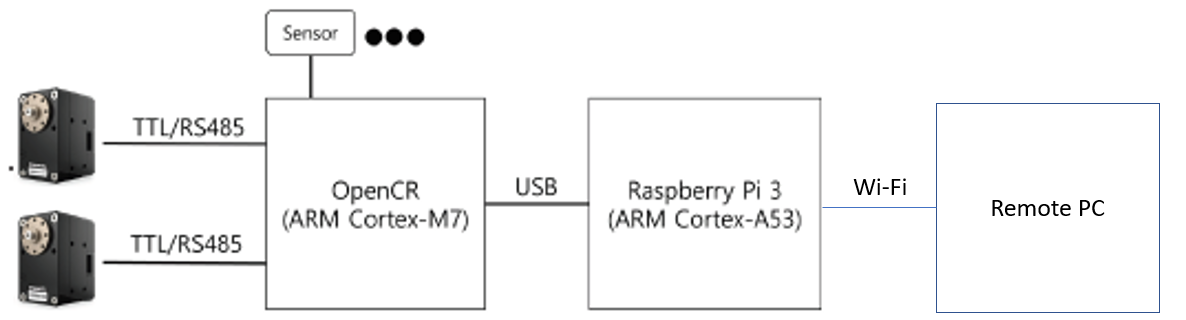
\includegraphics[width=0.7\linewidth]{images/tb3_architecture.png}\\
\end{center}
The four major components of \texttt{TurtleBot3} are 
\begin{enumerate}
	\item {Raspberry Pi 3B+ Single Board Computer (SBC).}
	\item {OpenCR Embedded System Board.}
	\item {LDS and Camera Sensors.}
	\item {Dynamixel Actuators.}
\end{enumerate}
Raspberry Pi has a WiFi module built onto the board which connects to a computer, known as the Remote PC. Remote PC is used to send goal waypoints for SLAM and Navigation to TB3. Visualization of the robot is also performed on the remote PC using a ROS-based tool called \texttt{rviz}.\\
There is a one time setup that needs to be performed on the Remote PC, Raspberry Pi and OpenCR board. The following sections detail the procedure to setup the software on various components.
%=====================================================================%
\subsection{Remote PC Setup}
%=====================================================================%
To begin you will need to install the appropriate ROS version on your remote PC. The remote PC will be running ROS Melodic (EOL date: May 2023).
\subsubsection{Quick Installation using Shell Script (recommended)}
A shell script \texttt{install\_melodic.sh} has been created to ease the installation of ROS and dependent packages on the Remote PC. This is located on the GitHub repo and can be cloned from there. Open a terminal and run the following commands.
\begin{lstlisting}[style=bash]
git clone https://github.com/hanyiabc/ACSL_turtlebot3.git
cd ASCL_turtlebot3/
chmod 755 ./install_melodic.sh && bash ./install_melodic.sh
\end{lstlisting}
If you face any errors that cannot be resolved, the \texttt{install\_melodic.sh} file is readable and you can execute those commands individually.
\subsubsection{Manual Installation of ROS Melodic}
If the shell script installation doesn't succeed, you can also follow instructions on ROS Wiki for setting up ROS Melodic on Ubuntu 18.04 manually. Complete the instructions on the following website.\\\\
\url{http://wiki.ros.org/melodic/Installation/Ubuntu}\\\\
Then, install required dependencies by running the last 3 commands in the \texttt{install\_melodic.sh} file. They can be easily found under the "Install Dependencies" section.\\
Finally clone the repository using the following commands.
\begin{lstlisting}[style=bash]
git clone https://github.com/hanyiabc/ACSL_turtlebot3.git
\end{lstlisting}
\subsubsection{Network Configuration}
Steps for configuring the wifi on the remote pc are taken from the following site and requirement specific instructions have been mentioned below.\\\\
\url {https://emanual.robotis.com/docs/en/platform/turtlebot3/pc_setup/#network-configuration}\\\\
For this project we will use the Linksys Router on the \textbf{Linksys04294} network. It is helpful to write down the IP address of the remote pc, since you will need it later to setup the turtlebot pc network settings.
\subsubsection{Compiling Source Code on Remote PC}
Once the network is setup on the Remote PC, go ahead and build the GitHub repository. This can be done by navigating to the top level folder of the repository \texttt{ASCL\_turtlebot3/} and running \texttt{catkin\_make} in the terminal.\\\\
Finally add the environment variable for the \texttt{TurtleBot3} model to \texttt{.bashrc} file and source it. Possible values are \textit{waffle, waffle\_pi, burger}. We have our own customized model and hence we have defined our own model name. Run the following commands to add the variables to the \texttt{.bashrc} file.
\begin{lstlisting}[style=bash]
echo "export TURTLEBOT3_MODEL=waffle_pi_effort_controller" >> ~/.bashrc
source ~/.bashrc
\end{lstlisting}
A different URDF file (an XML file for the ROS robot model) is loaded based on this environment variable. For this project however, we have defined new URDF file for effort control. By adding the above environment variable, ROS would use the appropriate file to model the robot for visualization and take the appropriate geometrical dimensions/parameters in the code.\\\\
This completes the Remote PC setup. It is advised to open \texttt{.bashrc} file using \texttt{Gedit} or any other text editor to make sure there are no duplicate commands being run. Having duplicates doesn't lead to any errors, but some variables might get redefined and it is not considered good practice to have multiple commands for setting up the same environment variables or aliases.
\subsection{Rasberry Pi SBC Setup}
The single board computer on \texttt{TurtleBot3} will be running ROS Kinetic (EOL date: April 2021) for the ease of setup since ROS Melodic requires manual compilation when using Rasbian. 
No problem has yet been found by us on the communication between these 2 releases.
Now it is time to look at the turtlebot SBC. For the turtlebot 3 Waffle Pi model, the on board PC is a raspberry PI. 
This step requires a micro SD card with adapter, a monitor with an HDMI input, a USB keyboard and mouse, and a power source for the turtlebot. 
ROBOTIS provides a prebuilt desktop environment for the turtlebot with ROS kinetic. Instructions for flashing this distribution can be found here. (\textbf{Step 6.2.1.2 Install Linux Based on Raspbian, Do not use the other two methods.}).\\\\
\url {https://emanual.robotis.com/docs/en/platform/turtlebot3/raspberry_pi_3_setup/#raspberry-pi-3-setup}\\\\
To use the Raspberry PI without a physical access, use SSH. Example SSH command:
\begin{lstlisting}[style=bash]
ssh pi@YOUR_RASPBERRY_PI_IP
\end{lstlisting}
For the ease of use, VNC configuration is recommended. This provide remote desktop funtionality. In case of Debian Stretch (the version that the manual will use), install Real VNC by running this command on the Raspberry PI:
\begin{lstlisting}[style=bash]
sudo apt update
sudo apt install realvnc-vnc-server realvnc-vnc-viewer
\end{lstlisting}
THen enable VNC server by 
\begin{lstlisting}[style=bash]
sudo raspi-config
\end{lstlisting}
Then navigate to Interfacing Options.
Scroll down and select VNC - Yes.


Ubuntu Desktop 18.04 comes with VNC client Remmina.
On Windows, use VNC viewer
\url{https://www.realvnc.com/en/connect/download/viewer/}
\subsection{OpenCR Setup}
Most of the software is located in the form of a binary file that is burnt to the EEPROM of the STM32F746 chip on the OpenCR board. As the software used for ACSL projects is custom, it is burnt using Arduino IDE.\\
The original source code for \texttt{TurtleBot3} used the inbuilt PID controller of the Dynamixel XM430 210-T actuators. However, to benchmark the performance of the controllers, the control is shifted from the motors to higher level software, which is a custom ROS PID node in this case.\\
Arduino IDE can be used to burn the \texttt{turtlebot3\_core.ino} file located in \texttt{ACSL\_turtlebot3/src/turtlebot3\_core} directory. Instructions for setting up the Arduino IDE for \texttt{TurtleBot3} can be found in the following link.\\\\
\url {https://emanual.robotis.com/docs/en/parts/controller/opencr10/#arduino-ide}\\\\
Once Arduino is setup, launch it and check if the port settings are correctly configured.
\begin{center}
	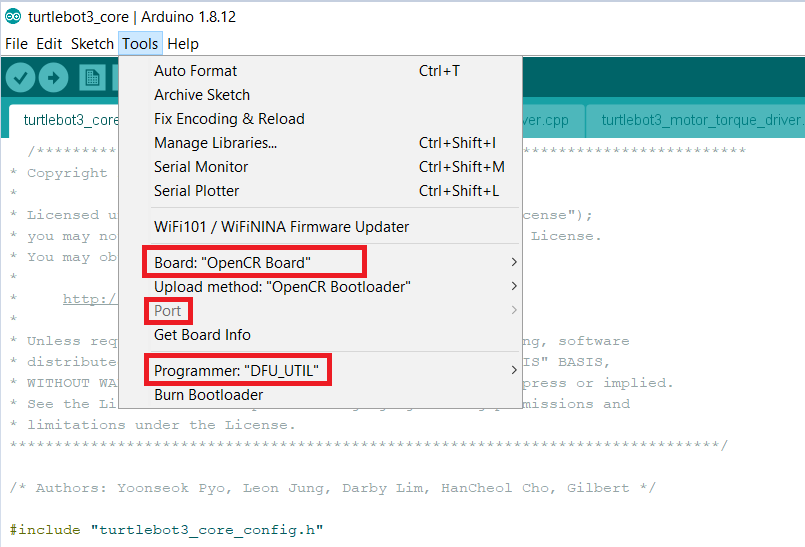
\includegraphics[width=0.5\linewidth]{images/arduino_setup.png}\\
\end{center}
Connect OpenCR via microUSB to the PC and flash the firmware using this button.\\
\begin{center}
	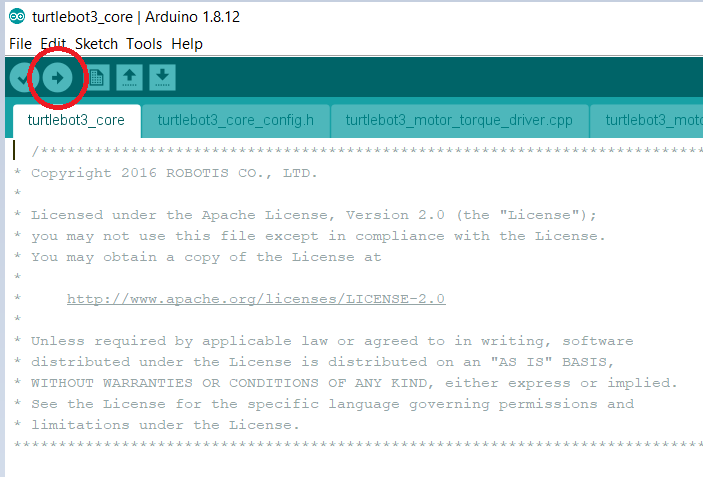
\includegraphics[width=0.5\linewidth]{images/arduino_flash.png}\\
\end{center}
\newpage
\section{Setting up Wireless File Sharing on an SBC Running Ubuntu}
This section is optional. If there are frequent changes to the OpenCR firmware then it makes more sense to flash it using the SBC. However, as there is no internet access in the lab for the TurtleBot SBC, the required binary files need to be transferred over WiFi. The software we will be using to share files via WiFi is called Samba. To install it follow these steps on the selected SBC.
\begin{lstlisting}
sudo apt update
sudo apt install samba
\end{lstlisting}
Next, pick the directory you would like to share and copy its path. In this example I will use the \textbf{/odroid/home} directory.
Now open the samba configuration folder. 
\begin{lstlisting}
sudo nano /etc/samba/smb.conf
\end{lstlisting}
Add the following to the end of the document. \textbf{"/odroid/home"} should be entered with the desired share directory.
\begin{lstlisting}
[sambashare]
comment = Samba on Ubuntu
path = /odroid/home
read only = no
browsable = yes
\end{lstlisting}
Press Ctrl-X, Y, and Enter to save.\\
Next add the firewall rules for Samba.
\begin{lstlisting}
sudo service smbd restart
sudo ufw allow samba
\end{lstlisting}
Finally setup a user for the Sambashare. This will need to match the name of an account already on the SBC. For this example I will use the \textbf{“Odroid”} user with password \textbf{1234}.
\begin{lstlisting}
sudo smbpasswd -a Odroid
Please Enter Password: 1234
Retype Password : 1234
\end{lstlisting}
The folder should now be accessible from any device on the same network. To access it go to \textbf{file manager, other locations} and enter this network address\\\\
smb://(ip-address of sbc)/sambashare\\\\
A prompt will appear for entering the user name and password you just setup.
\newpage
\section{Replacing the Raspberry Pi with an alternate SBC}
\subsection{Hardware Changes}
Before starting, you will need to attach an additional USB wi-fi device, as well as modify the OpenCR power output cable to fit the J5 barrel connector used by the Odroid. The 5v output port used for the Raspberry Pi will work for the Odroid if the connector is modified.\\\\
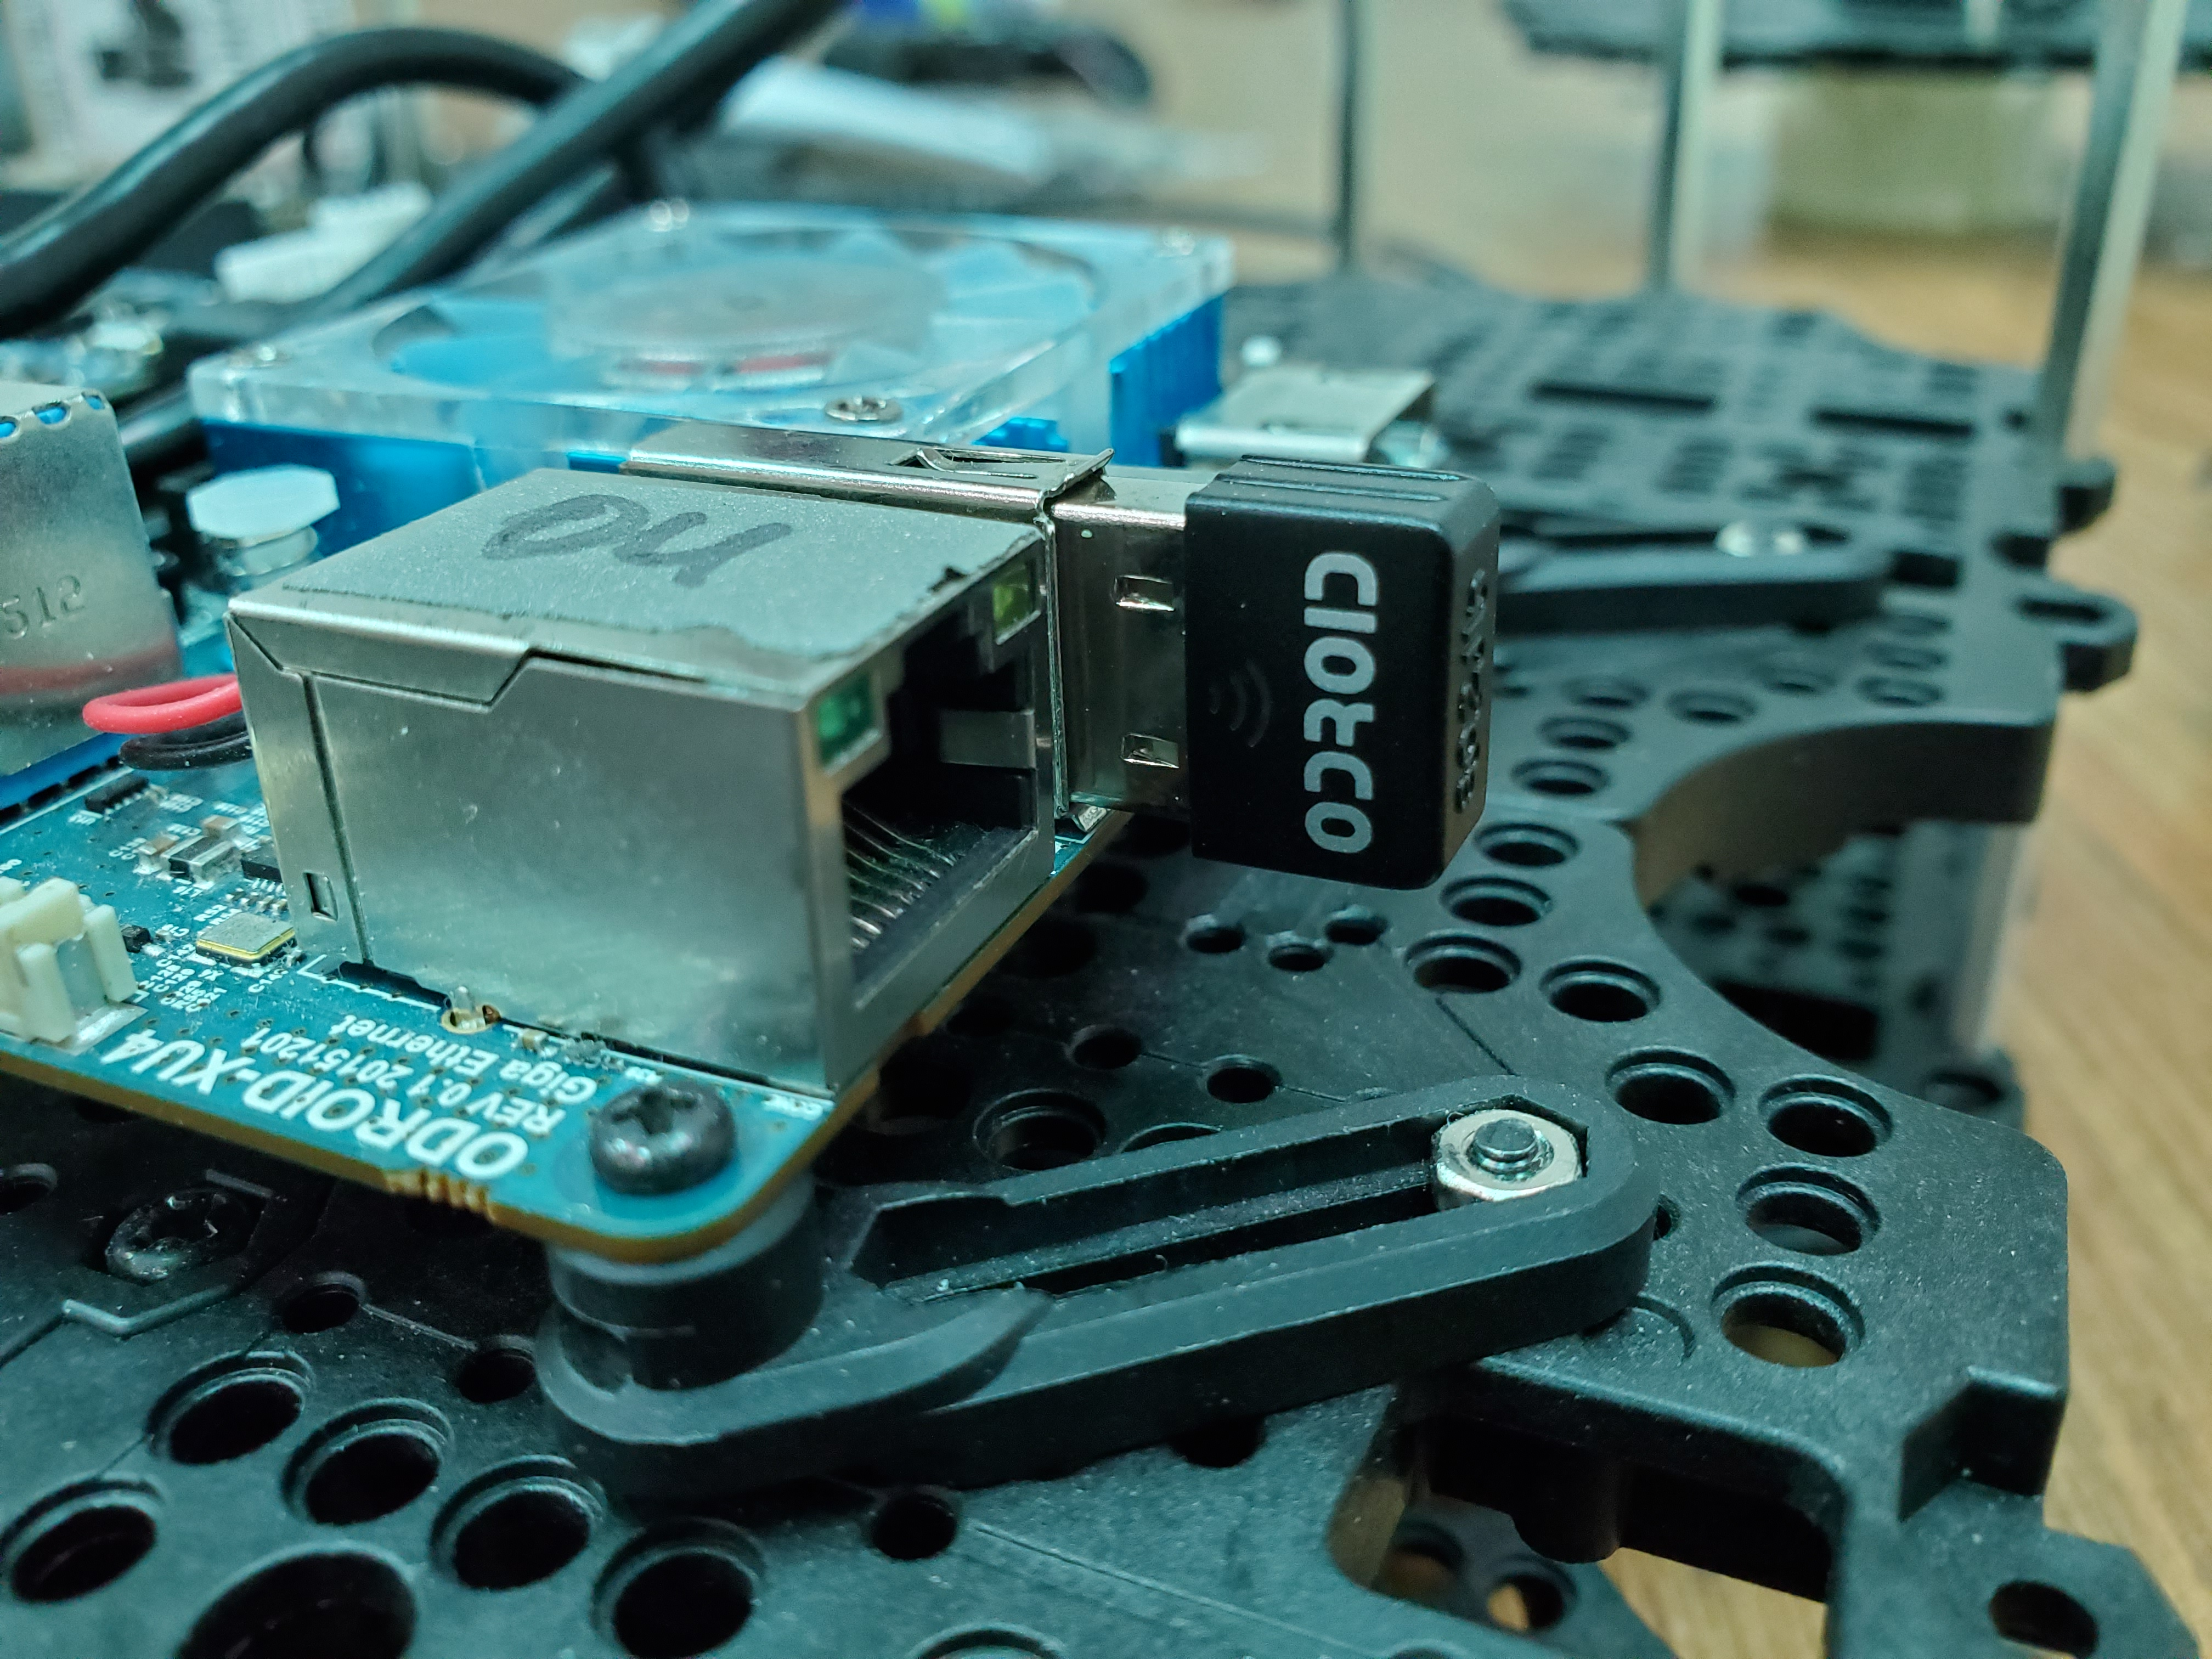
\includegraphics[width=0.5\linewidth]{images/WIFI_chip.jpg}
\includegraphics[width=0.5\linewidth]{images/DC_power_cable.jpg}\\
The Odroid XU4 has 2 modes for booting from memory. The micro SD card and the eMMMC memory chips. There is a switch near the power port for switching between these 2 modes\\
\begin{center}
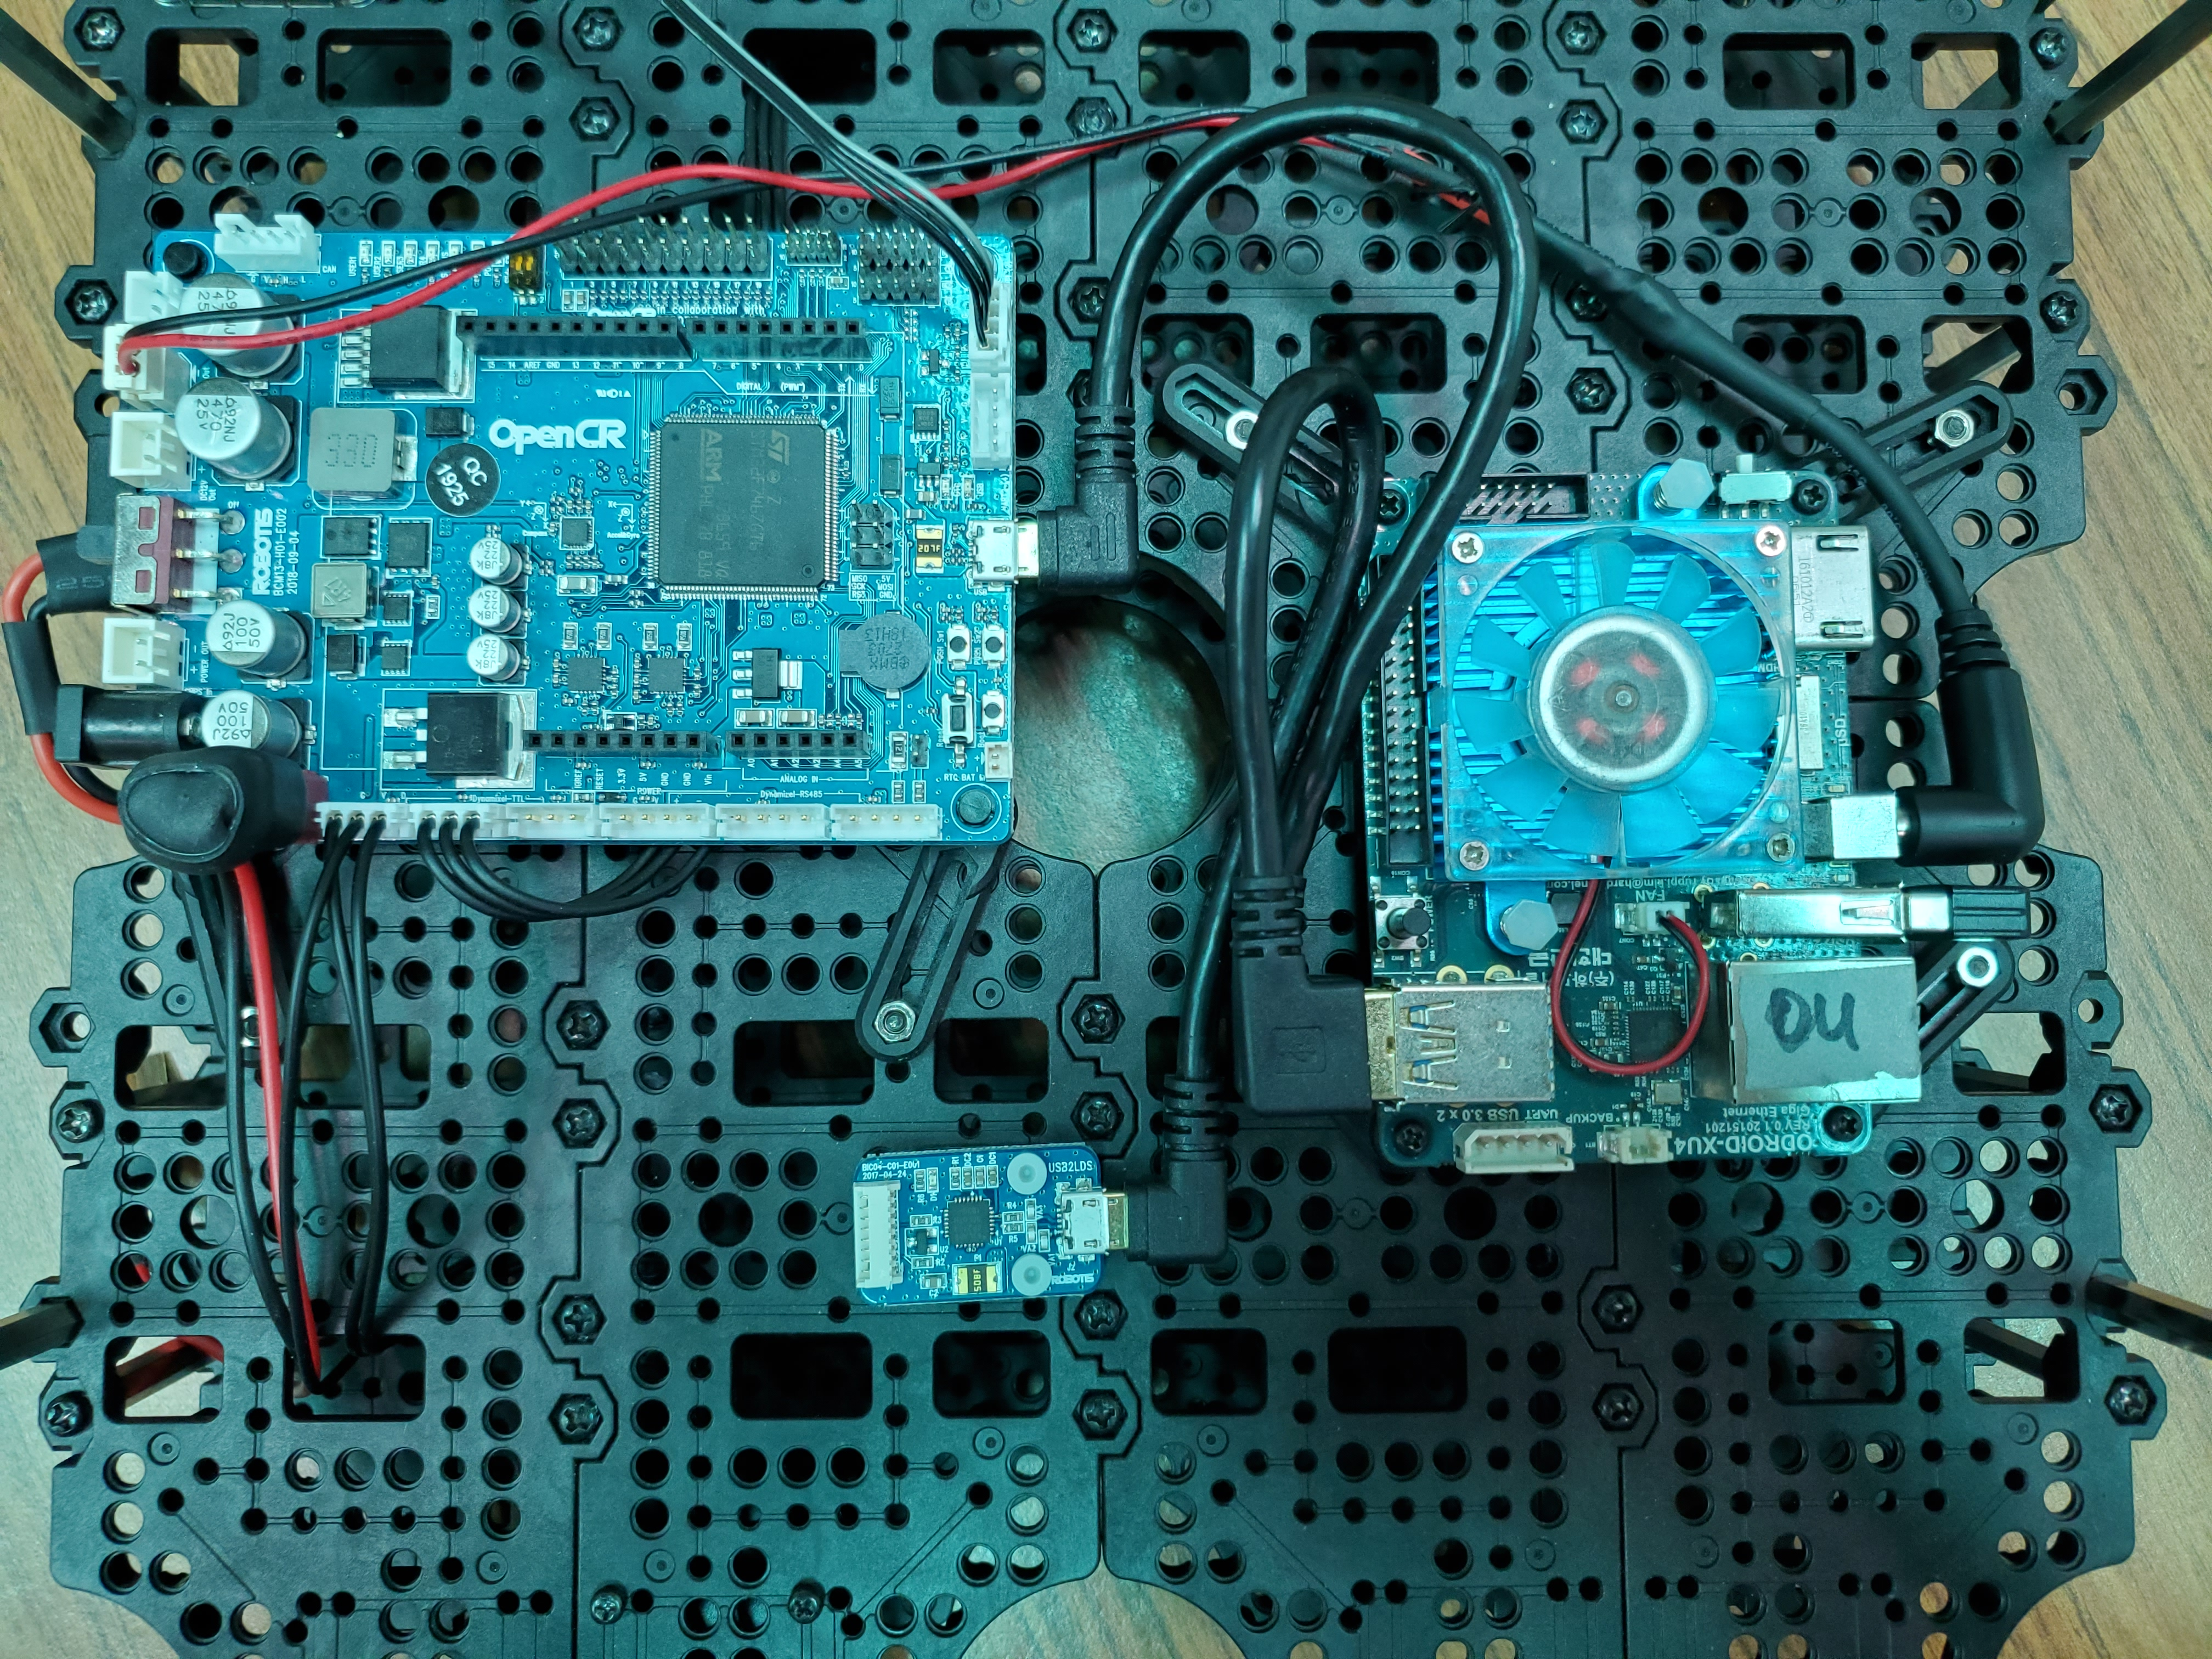
\includegraphics[width=0.75\linewidth]{images/ODROID_top.jpg}\\
\end{center}
\subsection{Software}
First you will need to flash a bootable ubuntu 16.04 OS onto the chosen memory device.\\
A suitable version can be found at\\\\
\url{https://odroid.in/ubuntu_16.04lts/}\\\\
We used the Ubuntu Mate version \textbf{ubuntu-16.04.3-4.9-mate-odroid-xu4-20171025.img.xz}\\
Connect the chosen memory device, and open a flash program such as Etcher and wait for flashing to finish.\\
After reconnecting the memory device, you can power up the Odroid. .The default user name is \textbf{Odroid}, and default password is also \textbf{Odroid}.\\
\subsection{ROS}
Follow the ROS wiki instructions for installing Ros-Kinetic.\\\\
\url{http://wiki.ros.org/kinetic/Installation/Ubuntu}\\\\
Next install the dependent packages using steps (3) through (5) of 6.2.1.1 Install Linux (Ubuntu MATE) from the turtlebot E-manual.\\
\url{https://emanual.robotis.com/docs/en/platform/turtlebot3/raspberry_pi_3_setup/#raspberry-pi-3-setup}\\\\
After finishing this step, you will be able to connect to the Odroid via SSH on the remote PC using the command line ssh odroid@192.168.xxx.xxx and using password odroid. 
%=====================================================================%
\newpage
\section{Syncing Time using NTP Server and Client}
%=====================================================================%
Raspberry Pi and Odroid SBCs do not have a hardware clock, and therefore it relies on an active internet connection to fetch the accurate time from Ubuntu time server. However, this is not possible as Linksys router, does not have internet access.\\
Every time SBC boots up, the time has to be updated. The time on the Remote PC and the SBC have to be synced up in order for the various transformations to work for the purpose of running SLAM and Navigation in the ACSL Lab Environment. Hence, to sync up time between these two machines, NTP protocol is being used.\\
NTP or Network Time Protocol is a protocol that is used to synchronize all system clocks in a network to use the same time. When we use the term NTP, we are referring to the protocol itself and also the client and server programs running on the networked computers. NTP belongs to the traditional TCP/IP protocol suite and can easily be classified as one of its oldest parts.\\
When you are initially setting up the clock, it takes six exchanges within 5 to 10 minutes before the clock is set up. Once the clocks in a network are synchronized, the client(s) update their clocks with the server once every 10 minutes. This is usually done through a single exchange of message(transaction). These transactions use port number 123 of your system.\\
In this section, a step-by-step procedure is described on how to:
\begin{itemize}
	\item{Install and configure the NTP server on a Ubuntu machine.}
	\item{Configure the NTP Client to be time synced with the server.}
\end{itemize}
These instructions are taken from \url{https://vitux.com/how-to-install-ntp-server-and-client-on-ubuntu/}. However, it is advised that the following instructions are followed as there are some project specific changes that have been made.
\subsection{Configure NTP Server on the Remote PC} 
Open Terminal and run the following commands \textbf{on the remote PC}
\begin{lstlisting}
	sudo apt-get update
	sudo apt-get install ntp
\end{lstlisting}
Most likely NTP will already be installed on the machine. After installation, the configuration file needs to be altered and server pools closest to the PC location needs to be added. This step is optional, as most likely the servers will be configured correctly.
\begin{lstlisting}
	sudo gedit /etc/ntp.conf
\end{lstlisting}
Replace/edit the server pools with the following.
\begin{lstlisting}
	pool 0.us.pool.ntp.org iburst
	pool 1.us.pool.ntp.org iburst
	pool 2.us.pool.ntp.org iburst
	pool 3.us.pool.ntp.org iburst
\end{lstlisting}
Save and close the configuration file. In order for the above changes to take effect, you need to restart the NTP server. The time from these servers will be synced with the time on the remote PC. as it has internet access. This will make sure that the NTP server clock is accurate.
\begin{lstlisting}
    sudo service ntp restart
\end{lstlisting}
Run the following command to check if the NTP server is configured properly. You should see the remote PC connecting to various servers.
\begin{lstlisting}
    sudo service ntp status
\end{lstlisting}
Finally, the system’s UFW firewall needs to be configured so that incoming connections can access the NTP server at UDP Port number 123. This is the most important step, as it will configure the remote PC to allow client connections.
\begin{lstlisting}
    sudo ufw allow from any to any port 123 proto udp
\end{lstlisting}
Now the Ubuntu host machine is configured to be used as an NTP server. Please take a note of the IP address of the remote PC \underline{when it is connected to the appropriate router.} IP address of a machine depends on which router it is connected to, and hence is not constant. We will need this address in the next step.
\subsection{Configure NTP Client on the SBC}
The \texttt{ntpdate} command will let you manually check your connection configuration with the NTP-server. Only in this case, the server would be the one that we specify. It should already be installed on the SBC, but in case it is not, run the following command \textbf{on the SBC}.
\begin{lstlisting}
    sudo apt-get install ntpdate
\end{lstlisting}
As the SBC will be a client to the host we set up on the remote PC, we need to modify the hosts file for NTP.
\begin{lstlisting}
    sudo gedit /etc/hosts
\end{lstlisting}
Now add your NTP server’s IP (remote PC IP address noted in the previous step) and specify a hostname. Assuming that the remote PC IP address is \texttt{192.168.1.183} and the server has to be named \texttt{ACSLServer}, add the following line to this file:
\begin{lstlisting}
    192.168.1.183	ACSLServer
\end{lstlisting}
Save and close the NTP hosts file. Because we want our client to sync time with the NTP server, the \texttt{timesyncd} service on the client machine needs to be disabled by running the following command.
\begin{lstlisting}
	sudo timedatectl set-ntp off
\end{lstlisting}
Now, we need to specify this NTP server on the remote PC in the NTP configuration file of the client. If \texttt{NTP} is not installed install it using the following command.
\begin{lstlisting}
	sudo apt-get install ntp
\end{lstlisting}
Now we want our client machine to use our own NTP host server to be used as the default time server. For this, we need to edit the \texttt{/etc/ntp.conf} file on the client machine.
\begin{lstlisting}
	sudo nano /etc/ntp.conf
\end{lstlisting}
Add the following line to the file before the list of other servers. There should be a comment indicating the location where new servers can be added, although this is only for readability and functionality shouldn't be affected.
\begin{lstlisting}
	server ACSLServer prefer iburst
\end{lstlisting}
Finally restart the \texttt{NTP} service and the time should be synced.
\begin{lstlisting}
	sudo service ntp restart
\end{lstlisting}
Now your client and server machines are configured to be time-synced. You can view the time synchronization queue by running the following command:
\begin{lstlisting}
ntpq -p
\end{lstlisting}
If \texttt{ACSLServer} is seen in the list of servers then the client is properly configured.\\
Finally the timezone needs to be set on the SBC to \texttt{America/New-York}. On the Odroid XU4 running \texttt{Ubuntu} with \texttt{MATE} desktop, it is a simple command line instruction as follows.
\begin{lstlisting}
	sudo timedatectl set-timezone America/New-York
\end{lstlisting}
This command may not work on the Raspberry Pi 3B+, but the timezone can be changed using the \texttt{raspi-config} utility.\\
Once the timezones are set, the SBCs are configured properly.
\newpage
\section{Bring up the Turtlebot}
Once the remote PC and Raspberry PI are setup according to the instructions provieded in the previous sections, 
Follow the instructions below to bring up turtlebot.  \\
On Remote PC
\begin{lstlisting}[style=bash]
    roscore
\end{lstlisting}
On SBC
\begin{lstlisting}[style=bash]
    roslaunch turtlebot3_bringup turtlebot3_robot.launch
\end{lstlisting}

On Remote PC, once you followed the instructions for building the workspace and setting up the environment variables,  
load the environment variables related to this workspace (Note: This has to be done everytime you want to run something from this workspace from a new termianl)
\begin{lstlisting}[style=bash]
cd ASCL_turtlebot3/
source devel/setup.bash
\end{lstlisting}

To run teleop to control the Turtlebot with keyboard.
\begin{lstlisting}[style=bash]
roslaunch turtlebot3_teleop turtlebot3_teleop_key.launch
\end{lstlisting}

To run the navigation with PID velocity effort controller and SLAM (with localizatin provided by SLAM and no initial map required) on the physical robot. 
\begin{lstlisting}[style=bash]
roslaunch turtlebot3_bringup turtlebot3_physical_nav_control.launch 
\end{lstlisting}

Note that the user might need to re-sync the time using NTP between the SBC and remote PC. Since SBC is not powered during shutdown, 
the time might be out of sync and this will cause error on the TF package from ROS since ROS uses time to track the transformations between each frames. Thus causing problem to the navigation stack. 
Simply do a manula update using NTP before lanuching will solve this issue.\\
To manually update the time and date using NTP (run this on the SBC instead of the remote PC and replace IP\_ADDRESS\_OF\_THE\_REMOTE\_PC with the IP address of the remote PC):

\begin{lstlisting}[style=bash]
    sudo ntpdate -u IP_ADDRESS_OF_THE_REMOTE_PC
\end{lstlisting}

To run the navigation with PID velocity effort controller and SLAM (with localizatin provided by SLAM and no initial map required) on Gazebo for simulation.  
\begin{lstlisting}[style=bash]
roslaunch turtlebot3_bringup turtlebot3_sim_nav_control.launch 
\end{lstlisting}

To run SLAM only to draw maps
Choose a pre-defined Gazebo world from the following:

\begin{itemize}
    \item[--] turtlebot3\_empty\_world.launch
    \item[--] turtlebot3\_world.launch
    \item[--] turtlebot3\_house.launch
    \item[--] turtlebot3\_stage\_1.launch
    \item[--] turtlebot3\_stage\_2.launch
    \item[--] turtlebot3\_stage\_3.launch 
    \item[--] turtlebot3\_stage\_4.launch
\end {itemize}
For example, if \textbf{turtlebot3\_world.launch} is chosen, run the following command to bring up a virtual Turtlebot on Gazebo for simulation
\begin{lstlisting}[style=bash]
roslaunch turtlebot3_gazebo turtlebot3_world.launch
\end{lstlisting}
\newpage
Then, run the following commands to launch the SLAM nodes and remote control using keyboard. 
\begin{lstlisting}[style=bash]
roslaunch turtlebot3_slam turtlebot3_slam.launch slam_methods:=gmapping
roslaunch turtlebot3_teleop turtlebot3_teleop_key.launch
\end{lstlisting}
Once you are satisfied with the map, save the map by running
\begin{lstlisting}[style=bash]
rosrun map_server map_saver -f ~/map
\end{lstlisting}
% TODO: Add figure from rqt_graph to illustrate topics and massages and connection between nodes, 
% TODO: add graph from tf view_frams to illustrate the TF tree 
\newpage
\section{Repository Introduction}
The repository is a catkin workspace. A catkin workspace has a src folder that contains multiple packages. The worth-mentioning ones are:
\begin{itemize}
	\item[--] hls\_lfcd\_lds\_driver
    \item[--] raspicam\_node
    \item[--] ros\_control
    \item[--] simulink
    \item[--] turtlebot3
    \begin{itemize}
        \item[--] turtlebot3\_bringup
        \item[--] turtlebot3\_navigation
        \item[--] turtlebot3\_slam
        \item[--] turtlebot3\_teleop
    \end {itemize}
    \item[--] turtlebot3\_core
    \item[--] turtlebot3\_setup\_motor
    \item[--] turtlebot3\_simulations
        \item[--] turtlebot3\_gazebo
\end{itemize} 

Not all packages are catkin package. \textbf{simulink}, \textbf{turtlebot3\_core} \textbf{turtlebot3\_setup\_motor} are all just directories. 
All the rests are properly configured as catkin packages, meaning all the nodes defined under the package will be compiled when running the \textbf{catkain\_make} command. 

\textbf{hls\_lfcd\_lds\_driver} and \textbf{raspicam\_node} are drivers for the PI Camera and lidar. 
These will be running in the single board computer. 

\textbf{ros\_control} contains all the configuration and nodes necessary to control the robot. 
It contains the PID controller configurationl, PID gains, etc.
Two launch files are included for controlling the robot in either the simulations or in the physical world. They are:

\begin{itemize}
	\item[--] turtlebot3\_control.launch
	\item[--] turtlebot3\_control\_simulation.launch
\end{itemize}  
These launch file are not ran directly, instead they are inlcuded by other launch file that we will introduce later.
The PID gains can be tuned by either changing the parameters in the launch file or use a ros package called rqt\_reconfigure to adjust parameters with sliders at runtime. 
There are 3 nodes under the \textbf{ros\_control} package. They are \textbf{differential\_driver.py}, \textbf{ros\_control\_odom\_pub} and \textbf{ros\_control\_node}. 
The \textbf{differential\_driver.py} is a Python ros node that split the incoming \textbf{\//cmd\_vel} messages into left and right velocity for the differential drive robot based on vehicle geometry. 
The \textbf{\/cmd\_vel} is the standard topic that ROS nav stack used to output the velocity command. It commands the robot in terms of translational velocity and orientation. 
The \textbf{ros\_control\_node} is a C++ ros node compiled from the soruce file: \textbf{message\_redirect.cpp}. 
This node simply takes the left and right wheel angular velocities feedbacks from \textbf{\/joint\_states} converts them to linear velocities and publish them into 2 Float64 messages for the PID controller to read.
The \textbf{ros\_control\_odom\_pub} is a C++ ros node compiled from the source file: \textbf{odom\_publisher.cpp}.

The directory \textbf{simulink} contains all the MATLAB scrips and Simulink models for controlling the robot with MATLAB (currently not uisng MATLAB). 

\textbf{turtlebot3\_bringup} contains all the launch file for bringing up the Turtlebot in the SBC and the remote PC. 
\textbf{turtlebot3\_physical\_nav\_control.launch} was added to the bringup package to provide a convinient one-file launch that will handles everything. 
This launch file brings up the turtlebot on the remote PC, runs the velocity control and the navigation stack with SLAM. A simulation version will be provided in the future.

\textbf{turtlebot3\_description} contains the URDF and Gazebo descripion of the turtlebot for both simulation and physical robot. 

For Waffle Pi, \textbf{turtlebot3\_waffle\_pi.gazebo.xacro}
and \textbf{turtlebot3\_waffle\_pi.urdf.xacro}
are provided by the turtlebot package, however, for effort control, we added 2 more files. 
They are: \\
\textbf{turtlebot3\_waffle\_pi\_effort\_controller.gazebo.xacro}
and \textbf{turtlebot3\_waffle\_pi\_effort\_controller.urdf.xacro}
These files are derived from the original descriptions and added ability to control effort in both the simulation and the physical robot. 

\textbf{turtlebot3\_navigation} contains the default configuration for running the ROS navigation stack with the Turtlebot.
A new launch file \textbf{turtlebot3\_navigation\_no\_map.launch} was created. This launch file derived from the original navigation launch file, but the difference is that this configuration doesn't need a SLAM map for localizatin. 
The localizatin is provide by SLAM instaed of Adaptive Monte Carlo Localizatin. The default launch file \textbf{turtlebot3\_navigation.launch} will run navigation assuming that a SLAM map has been drawn by running SLAM before. In this configuration, 
localizatin is provided by AMCL. 

\textbf{turtlebot3\_slam} contains all the configurations and launch files related to running SLAM. 
Several SLAM algorithms are pre-configured and supporeted but only Gmapping and *Cartographer are tested, feel free to test other SLAM algorithms. \\
\textbf{turtlebot3\_teleop} containes the node and launch file necessary for keyboard teleop (using keyboad to control the turtlebot). \\
\textbf{turtlebot3\_core} derives from the original package from the OpenCR library. This is an Arduino sketch and this program is running in the OpenCR microcontroller. This package handles every low-level operation of the physical turtlebot.
That includes reading sensor information, commanding motor torque, reading encoder information, etc. \\

\textbf{turtlebot3\_setup\_motor} is also an Arduino sketch that needs to run on the microcontroller, however, 
this only need to be ran once for each new set of Turtlebot motors. 
This package derives from the original turtlebot3\_setup\_motor from the OpenCR library. The original library sets the servos to velocity control operating mode. 
This package added the options to set the servos to torque control opearting mode. \\

\textbf{turtlebot3\_gazebo} in located under \textbf{turtlebot3\_simulations}. This package contains all the Gazebo related files necessary for running simulation with Gazebo. 
It contains a few pre-configured Gazebo world and 3D model for each model of the turtlebot. 

Note: we are encoutering problems running Cartographer with Turtlebot because it enforces a timestamp constraint on the incoming messages. 
The IMU messages in particular could have same timestamp in 2 consecutive messages, which caues the Cartographer node to throw an exception. 
A potential fix is to change the source code of Cartographer and make it use "more than or equal" to check the timestamp instead of using "more than".
Gmapping works totally fine for us. We have only faced these issue when running SLAM with no initial map and with SLAM's built-in localization. 
We expect that the problems will be gone once we use SLAM for mapping only and then save the map, the uses AMCL for localizatin. 

\section{Torque Control using Dynamixel}
       
Dynamixel is a microcontroller based actuator with in-built PID controller. OpenCR communicates with Dynamixel using packet communication via TTL/RS45 ports. 

Hardware level abstraction is achieved via Dynamixel SDK library available in several programming languages. (CPP used in our case.)
Dynamixel register addresses and byte sizes for both RAM and EEPROM memory provided in control table. RAM is most frequently used memory for robot applications, while startup settings are stored on EEPROM.

The Control Table is a structure that consists of multiple Data fields to store status or to control the device. Users can check current status of the device by reading a specific Data from the Control Table with Read Instruction Packets. WRITE Instruction Packets enable users to control the device by changing specific Data in the Control Table. Packet sizes range from 1 – 4 bytes.

Following is a snapshot of the Dynamixel EEPROM Control Table. Each data in the Control Table is restored to initial values when the device is turned on. Default values in the EEPROM area (addresses 0-63) are initial values of the device (factory default settings). If any values in the EEPROM area are modified by a user, modified values will be restored as initial values when the device is turned on. Initial Values in the RAM area are restored when the device is turned on.

\begin{center}
	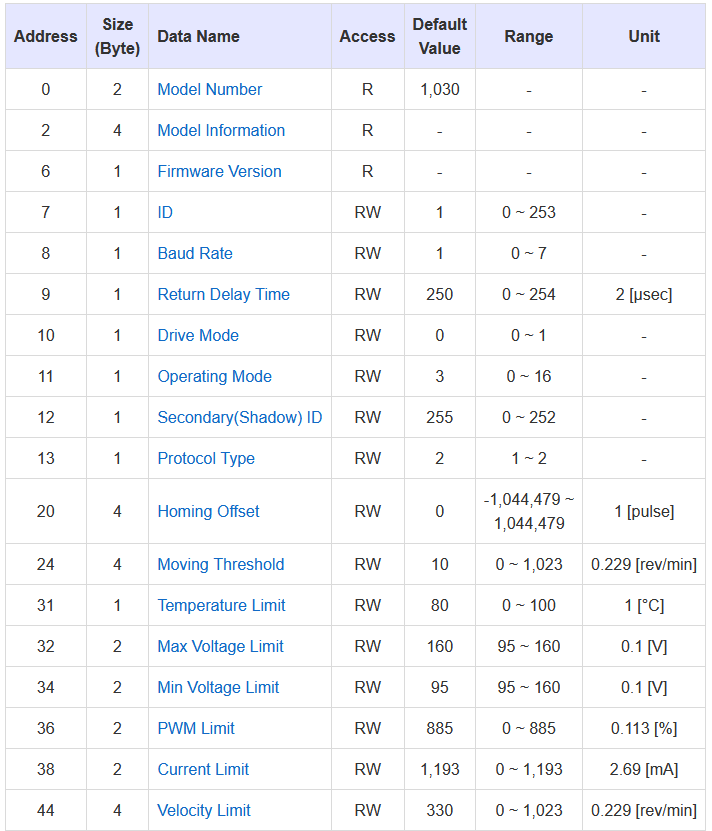
\includegraphics[width=0.7\linewidth]{images/dxl_eeprom.png}\\
\end{center}

For the purpose of torque control, the operating mode of the dynamixel motor needs to be set to \textbf{MODE 0}. This can be done using the motor setup code in the git repository.
To change the operating mode to \textbf{MODE 0}, flash the turtlebot3\_setup\_motor firmware to the OpenCR board while the motors are connected to the board. 
Open up a serial terminal with Arduino or Terraterm, under the serial termianl, you will see the following options:
\begin{lstlisting}[style=bash]
    1. setup left  motor
    2. setup right motor
    3. test  left  motor
    4. test  right motor
    5. setup left  motor for current control
    6. setup right  motor for current control
    7. test left  motor for current control
    8. test right  motor for current control
>> 
\end{lstlisting}
The first 4 options comes with the OpenCR Arduino library. The last 4 options are added based on the first 4 options and they configure the left and right motors for torque control.
For now, the current is limited to half of the highest value to avoid damage to the hardware. If changes are needed, the source code needs to be modified and the motors has to be setup again. 
To setup the left motor, simply put 5 in the termianl and press enter. Wait until it says it's finished. Then use option 6 for the right motor.
After the setup is done, use option 7 and 8 to test the motor. The test option apply a small torque to the motor for one second and stops for one second. Make sure both motors are tested then, flash the turtlebot3\_core firmware back.
Once the operating mode is set. The OpenCR code is changed to write torque values to the Dynamixel RAM addresses, when the robot is live. The addresses that are useful for this purpose are given in the image below.

\begin{center}
	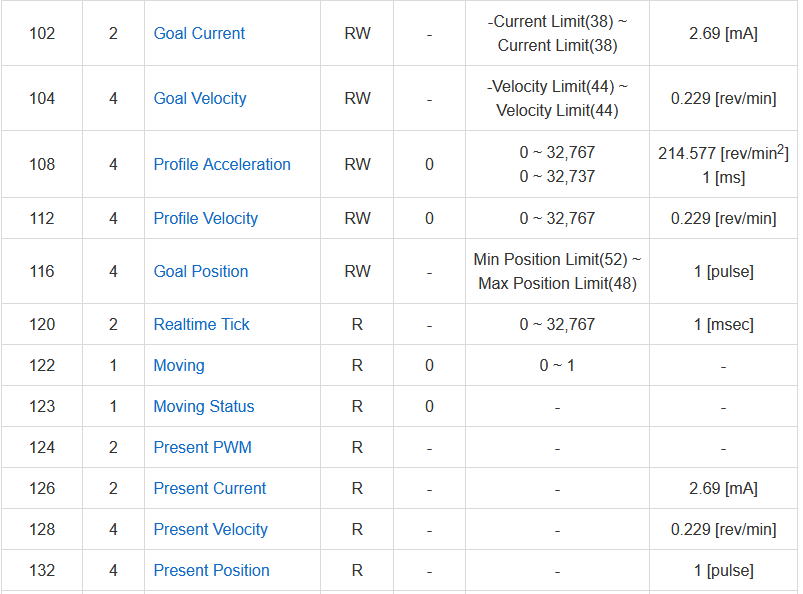
\includegraphics[width=\linewidth]{images/dxl_control_table.png}\\
\end{center}

The code that change the operating mode of the motor is below. 

\lstinputlisting[style=C++, firstline=511, lastline=561]{../src/turtlebot3_setup_motor/turtlebot3_setup_motor.ino}

The code used to test the torque control after setup is below. 
\lstinputlisting[style=C++, firstline=453, lastline=510]{../src/turtlebot3_setup_motor/turtlebot3_setup_motor.ino}

The OpenCR Arduino library comes with a TurtleBot3MotorDriver class that helps controlling the 2 motors by commanding velocities. 
A new class TurtleBot3MotorTorqueDriver was derived (strictly speaking, not inherited, instead just copied and pasted) from the TurtleBot3MotorDriver with new member functions added for controlling the torque instead of velocities. 
The class is defined as below
\lstinputlisting[style=C++, firstline=38, lastline=74]{../src/turtlebot3_core/turtlebot3_motor_torque_driver.h}

The following member functions is added to the TurtleBot3MotorDriver class, which takes in input torque value and converts it into appropriate register values for writing to the appropriate addresses.
\lstinputlisting[style=C++, firstline=275, lastline=291]{../src/turtlebot3_core/turtlebot3_motor_torque_driver.cpp}

\textbf{CURRENT\_TO\_OUTPUT} and \textbf{TORQUE\_TO\_CURRENT} are macro functions that does the conversions from torque to current and current to a 2 byte value that the microcontroller undertand. 
All the necessary macros are defined as
\lstinputlisting[style=C++, firstline=23, lastline=36]{../src/turtlebot3_core/turtlebot3_motor_torque_driver.h}

This conversion is based on a linear approximation of the actuator performance graph.

\begin{center}
	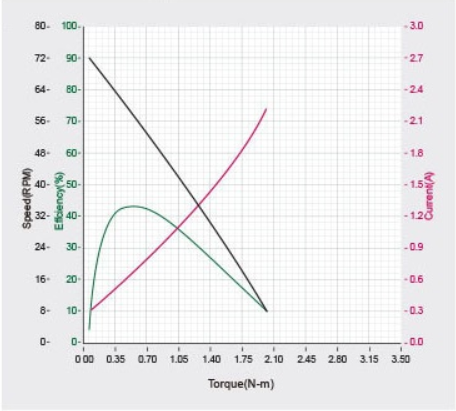
\includegraphics[width=\linewidth]{images/xm430_performance.png}\\
\end{center}

This function below takes the converted value and write to both motors using the Dynamixel SDK APIs. 
\lstinputlisting[style=C++, firstline=227, lastline=249]{../src/turtlebot3_core/turtlebot3_motor_torque_driver.cpp}

Subscribers are added to subscribe to the topics \/left\_torque \/right\_torque. 
The following use the function defined above and write the correspounding values to the correct memory location of the Dynamixel motor controller when new message comes in. 
When there is no new message, it will timeout and write zeros to both motors. 

\lstinputlisting[style=C++, firstline=87, lastline=99]{../src/turtlebot3_core/turtlebot3_core.ino} 
This Python node will convert the cmd\_vel to the left and right velocities command based on the robot geometry. 

\lstinputlisting[style=Python]{../src/ros_control/src/differential_driver.py}

The original Odometry publisher is in the microcontroller. Since the built-in differential drive plugin which provides 
Odometry that's used in the simulation was replaced by our own controller,
An Odometry publisher was added to the system to provide the Odometry in the simulation only. The source code is below. 

\lstinputlisting[style=C++]{../src/ros_control/src/odom_publisher.cpp}

This program is adapted from the Odometry publisher on the microcontroller. It takes the information from the simulated IMU and joint states to generate Odometry messages
for simulation. The orientation is taken from the imu and the position is taken from the joint states. It also publishes the transformations between the
base frame and the Odometry frame. The covariance matrix in the Odometry messgae is ignored and its elements are all 0s. \\

To control the left and right wheel joint using effort command in the simulation, the URDF and Gazebo descriptions of the robot are also modified as follow. \\

\textbf{src/turtlebot3/turtlebot3\_description/urdf/turtlebot3\_waffle\_pi\_effort\_controller.urdf.xacro:} \\
\lstinputlisting[style=XML, firstline=219, lastline=239]{../src/turtlebot3/turtlebot3_description/urdf/turtlebot3_waffle_pi_effort_controller.urdf.xacro}

\textbf{src/turtlebot3/turtlebot3\_description/urdf/turtlebot3\_waffle\_pi\_effort\_controller.gazebo.xacro:} \\
\lstinputlisting[style=XML, firstline=11, lastline=31]{../src/turtlebot3/turtlebot3_description/urdf/turtlebot3_waffle_pi_effort_controller.gazebo.xacro}
\lstinputlisting[style=XML, firstline=61, lastline=88]{../src/turtlebot3/turtlebot3_description/urdf/turtlebot3_waffle_pi_effort_controller.gazebo.xacro}

A configuration file was added to make commanding effort to left and right wheel joints in Gazebo simulation possible\\
\textbf{/src/ros\_control/params/bot\_control.yaml} \\

\section{Turtlebot Graphical User Interface}
This section documents the graphical user interface for manipulating the TurtleBot3 in both real world and simulated environments. It contains descriptions for each graphical widget and code documentation. The turtlegui package contains all of the c++ scripts and dependency files responsible for the interface. And once the package is appropriately sourced via the terminal, it can be run with the following command:\\

\begin{lstlisting}[style=bash]
rosrun turtlegui turtlegui
\end{lstlisting}
\subsection{Qt}
The interface runs on Qt, a cross-platform graphical toolkit. 
This module implements a variety of important classes, the first of which is QApplication. 
The source code for the instantiation of the Turtlebot qt application, in main.cpp, is

\lstinputlisting[style=C++, firstline=20, lastline=32]{../src/turtlegui/src/main.cpp}
The QApplication class takes care of a lot of things, most notably the input CLI arguments and the event loop. The event loop is a loop that waits for user input in GUI applications, and is launched on this command

\lstinputlisting[style=C++, firstline=29, lastline=29]{../src/turtlegui/src/main.cpp}
Another important Qt class is QWidget, which is used to describe the widgets in the interface. Widgets are the basic building blocks for a GUI application, and are able to respond to user events. All of the graphical elements in the interface inherit from the QWidget class, including QPushButton, QRadioButton, and QLineEdit. Widgets are also responsible for the handling of the signal and slot mechanism. On a high level, signals and slots are used for communication between objects. In GUI programming, when one widget changes, other widgets need to be notified of this change. Rather than hard-wiring the code that generates these events, signals and slots allow for fluid communication between objects.\\ 

As seen in the line of code below, the lastWindowClosed() signal connects to the quit() slot so that when the exit button is clicked in the GUI, the program terminates.
\lstinputlisting[style=C++, firstline=28, lastline=28]{../src/turtlegui/src/main.cpp}
The Qt toolkit is a very useful module for handling the front-end side of programming and allows for a seamless transition to back-end code.

\subsection{GUI Widget Walkthrough}
This section gives a detailed description for each widget in main window of the interface. A screenshot of the interface can be seen below
\begin{center}
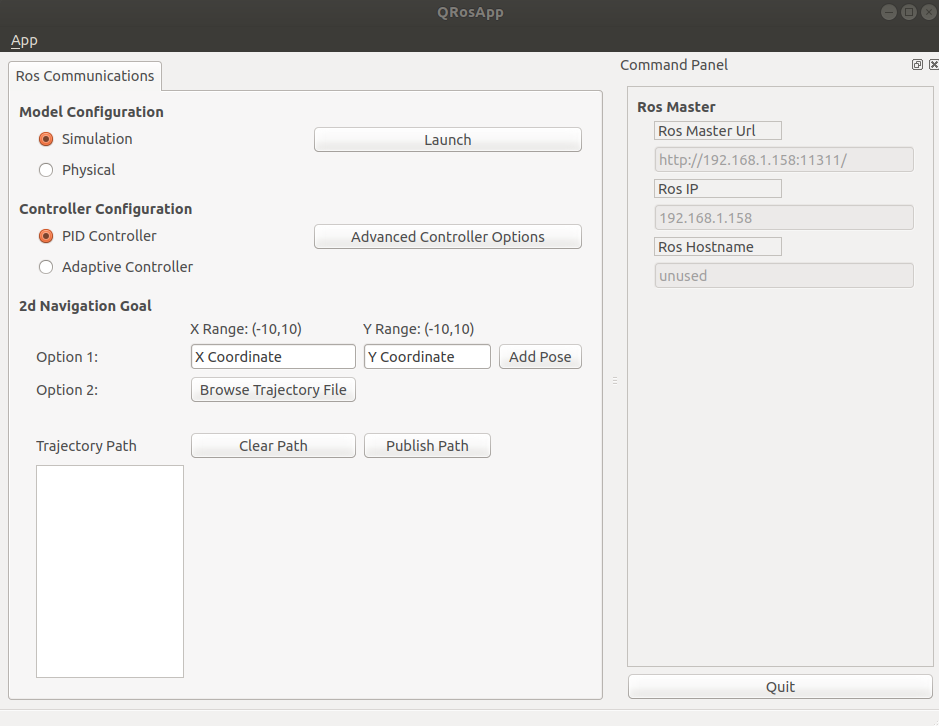
\includegraphics[width=0.9\linewidth]{images/gui_screenshot.png} \\
\end{center}
On startup, a ROS Master is initialized, this provides naming and registration services to the rest of the nodes in the ROS system. It tracks publishers and subscribers to topics as well as services. The role of the Master is to enable individual ROS nodes to locate one another. Once these nodes have located each other they communicate with each other peer-to-peer. All ROS commands are handled implicitly, thus requiring a single terminal window.\\

The three main sections of the GUI are Model Configuration, Controller Configuration, and 2d Navigation Goal.\\

\subsubsection{Model Configuration}
The first tab contains two QRadiobuttons and one QPushButton that allow the user to specify and launch an environment for the Turtlebot. The simulation launches Gazebo and RVIZ instances for visualization. This is accomplished by running this ROS command:
\lstinputlisting[style=C++, firstline=156, lastline=157]{../src/turtlegui/src/main_window.cpp}
The ROS launch command is blocking, which means once it is executed, another terminal window must be opened to run any additional commands. The ampersand at the end of the command tells the process to run in the background, allowing for more commands to be run in the same window. The real-world option uses the same syntax but launches a different package:
\lstinputlisting[style=C++, firstline=156, lastline=157]{../src/turtlegui/src/main_window.cpp}

Once an environment is loaded, never before, the dynamics and path of the turtlebot can be manipulated as seen in the following sections. Since there are multiple ROS processes running in the same terminal, ROS has trouble shutting them all down properly and tends to stall the terminal. In order to expedite the shutdown, the timeout time specified in following file was modified:

\begin{lstlisting}[style=bash]
/opt/ros/melodic/lib/python2.7/dist-packages/roslaunch/nodeprocess.py
\end{lstlisting}

\subsubsection{Controller Configuration}
This section allows the user to manipulate the parameters of the turtlebot. Again it contains two QRadiobuttons and one QPushButton for configuring the controller for the Turtlebot. It is important to note that only the PID controller option has been implemented, the Adaptive Controller does not do anything. The update controller parameters button runs on rqt, a software framework of ROS that implements the various GUI tools in the form of plugins. More specifically it uses an rqt metapackage called rqt\_gui, which allows multiple rqt plugins to be docked in a single window. The command that handles the instantiation and reference to this framework is:
\lstinputlisting[style=C++, firstline=162, lastline=163]{../src/turtlegui/src/main_window.cpp}
This launches a new window for viewing all ROS nodes and topics, configuring the PID parameters, and graphically analyzing the error of the PID controller. 
A screenshot of the window is shown below
\begin{center}
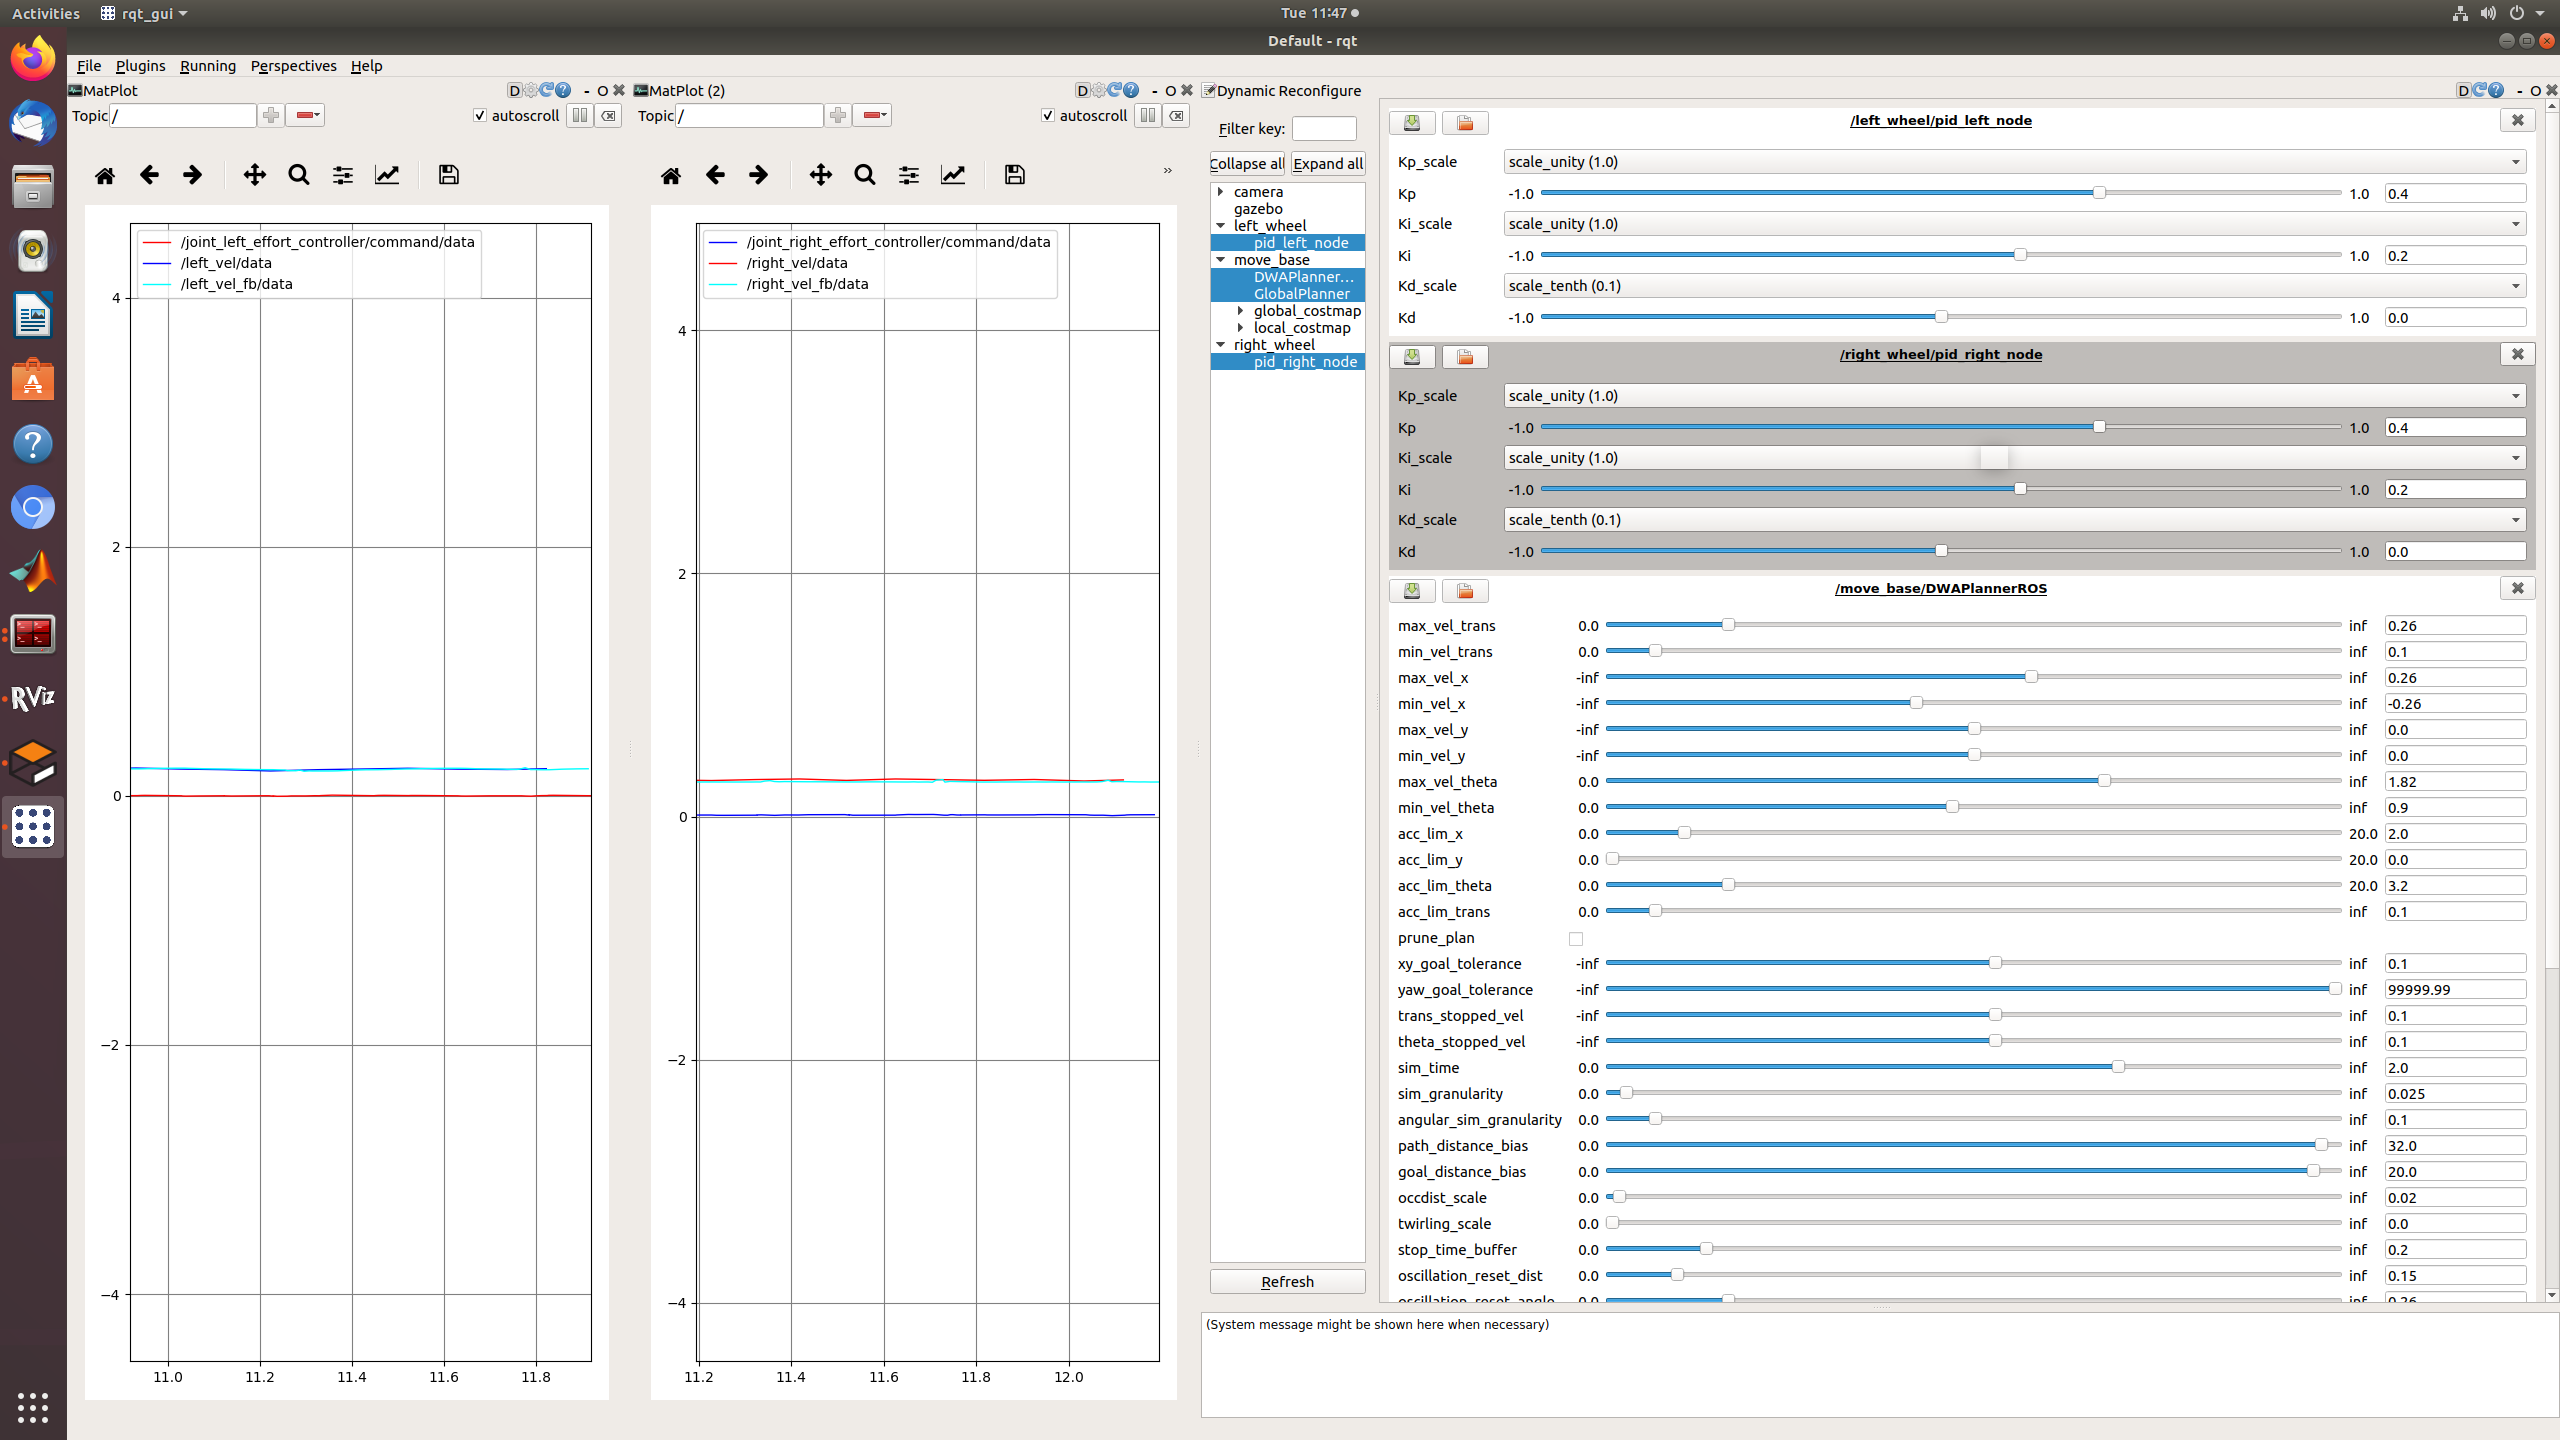
\includegraphics[width=0.9\linewidth]{images/rqt_gui.png} \\
\end{center}

\subsubsection{2d Navigation Goal}

Note that on a new computer, when rqt\_gui run in the first time, it will be a blank screen, 
the user would have to import a perspective manually to load this pre-configured perspective.
Simply follow the steps below to load the perspective: \\
From the turtlegui, select "Simulation" then click "Launch"\\
Click "Advanced Controller Parameters"\\
In the rqt\_gui windows that poped-up, click "Perspective" on the top menu bar, 
then click Import to browse for \textbf{rqt\_gui.perspective} located under the root of the ros workspace. \\


The turtlebot is able to follow one or more precise waypoints specified by the user via the 2D Navigation Goal section of the interface. 
Option 1 allows for the publishing of a single waypoint while option 2 lets the user browse for a csv file containing a list of waypoints. 
The trajectory path inherits the QStringListModel class that keeps track of the robot's current path. 
Once either option is chosen, the trajectory path will be updated. 
The clear\_path button simply removes all items from the trajectory path. 
To get the Turtlebot to actually start moving and following the path, the publish\_path button must be pressed.\\ 

This button utilizes the follow\_waypoints package, which handles the low-level robot communication for following a path. 
Three critical ROS commands are executed, the first of which can be seen below.

\lstinputlisting[style=C++, firstline=82, lastline=83]{../src/turtlegui/src/main_window.cpp}

This creates three ROS topics, /initialpose, /path\_ready, and /path\_reset. 
The /path\_reset topic is published when the clear path button is clicked. 
The input trajectory path is published to the /initialpose topic. 
This topic is of type geometry\_msgs/PoseWithCovarianceStamped, 
thus the messages published to this topic have to be of this type. 
This message type contains two fields, std\_msgs/Header header and geometry\_msgs/PoseWithCovariance pose. 
The former field is just used for communicate timestamped data in a particular coordinate frame. 
The latter has two more implicit fields, geometry\_msgs/Pose pose and float64[36] covariance. 
The pose field represents a pose in free space with uncertainty. 
The covariance field is a row-major representation of the 6x6 covariance matrix, which specifies the uncertainty of the pose field. 
The pose field has two more implicit fields, geometry\_msgs/Point position and geometry\_msgs/Quaternion orientation. 
The former contains the position of a point in free space, with fields: float64 x, float64 y, float64 z. 
The latter represents an orientation in free space in quaternion form, with fields float64 x, float64 y, float64 z, float64 w. 
By default, the covariance, orientation, and pose.z are all zero, thus the user only needs to specify an x and y position. 
It is important to note that if the specified goal is not close to current position of the Turtlebot, it will not move. 
The trajectory.csv file can be used to get an idea of the coordinate pairs the Turtlebot will be able to move to.\\

Once the path is published, another ROS command is executed:
\lstinputlisting[style=C++, firstline=89, lastline=89]{../src/turtlegui/src/main_window.cpp}
This just publishes an empty message to /path\_ready which tells the Turtlebot to start following the path published to /initialpose. Once the Turtlebot reaches the last point in the path, it will stop moving and a new path will have to be specified. The Turtlebot always starts at the origin, and its position is continuously published to the /odom ROS topic. 

\newpage
\section{List of ROS Nodes, Topics, Parameters, Transform}
\subsection{List of Important ROS Nodes}


% TODO: Mising a few
\begin{itemize}
    \item[--] /differential\_driver 
    \item[--] /left\_wheel/pid\_left\_node
    \item[--] /message\_redirect (used for generating PID feedback)
    \item[--] /move\_base (navigation stack node)
    \item[--] /odom\_pub (simulation only)
    \item[--] /right\_wheel/pid\_right\_node
    \item[--] /robot\_state\_publisher
    \item[--] /rviz
    \item[--] /turtlebot3\_slam\_gmapping (name will be changed based on the SLAM algorithm) 
    \item[--] /follow\_waypoints (node for following waypoints)
    \item[--] /turtlebot\_3\_core (physical robot only)
\end{itemize} 

\subsection{List of Topics and Their Types}

\begin{itemize}
\item[--] /map\_metadata [nav\_msgs/MapMetaData]
\item[--] /camera/rgb/image\_raw [sensor\_msgs/Image]
\item[--] /move\_base/current\_goal [geometry\_msgs/PoseStamped]
\item[--] /move\_base/local\_costmap/footprint [geometry\_msgs/PolygonStamped]
\item[--] /tf [tf2\_msgs/TFMessage]
\item[--] /move\_base/local\_costmap/costmap [nav\_msgs/OccupancyGrid]
\item[--] /odom [nav\_msgs/Odometry]
\item[--] /joint\_left\_effort\_controller/command [std\_msgs/Float64]
\item[--] /scan [sensor\_msgs/LaserScan]
\item[--] /left\_vel\_fb [std\_msgs/Float64]
\item[--] /camera/rgb/image\_raw/compressed [sensor\_msgs/CompressedImage]
\item[--] /left\_wheel/pid\_left\_node/parameter\_updates [dynamic\_reconfigure/Config]
\item[--] /move\_base\_simple/goal [geometry\_msgs/PoseStamped]
\item[--] /move\_base/DWAPlannerROS/cost\_cloud [sensor\_msgs/PointCloud2]
\item[--] /move\_base/DWAPlannerROS/trajectory\_cloud [sensor\_msgs/PointCloud2]
\item[--] /tf\_static [tf2\_msgs/TFMessage]
\item[--] /imu [sensor\_msgs/Imu]
\item[--] /map [nav\_msgs/OccupancyGrid]
\item[--] /move\_base/global\_costmap/footprint [geometry\_msgs/PolygonStamped]
\item[--] /joint\_right\_effort\_controller/command [std\_msgs/Float64]
\item[--] /cmd\_vel [geometry\_msgs/Twist]
\item[--] /move\_base/DWAPlannerROS/local\_plan [nav\_msgs/Path]
\item[--] /waypoints [geometry\_msgs/PoseArray]
\item[--] /joint\_states [sensor\_msgs/JointState]
\item[--] /move\_base/goal [move\_base\_msgs/MoveBaseActionGoal]
\item[--] /initialpose [geometry\_msgs/PoseWithCovarianceStamped]
\item[--] /rosout\_agg [rosgraph\_msgs/Log]
\item[--] /move\_base/GlobalPlanner/plan [nav\_msgs/Path]
\item[--] /move\_base/DWAPlannerROS/global\_plan [nav\_msgs/Path]
\item[--] /left\_vel [std\_msgs/Float64]
\item[--] /right\_wheel/pid\_debug [std\_msgs/Float64MultiArray]
\item[--] /camera/rgb/image\_raw/compressedDepth [sensor\_msgs/CompressedImage]
\item[--] /camera/rgb/camera\_info [sensor\_msgs/CameraInfo]
\item[--] /camera/rgb/image\_raw/theora [theora\_image\_transport/Packet]
\item[--] /gazebo/link\_states [gazebo\_msgs/LinkStates]
\item[--] /move\_base/GlobalPlanner/potential [nav\_msgs/OccupancyGrid]
\item[--] /gazebo/model\_states [gazebo\_msgs/ModelStates]
\item[--] /clock [rosgraph\_msgs/Clock]
\item[--] /right\_vel\_fb [std\_msgs/Float64]
\item[--] /move\_base/cancel [actionlib\_msgs/GoalID]
\item[--] /right\_vel [std\_msgs/Float64]
\item[--] /move\_base/global\_costmap/costmap [nav\_msgs/OccupancyGrid]
\item[--] /left\_torque [std\_msgs/Float64]
\item[--] /right\_torque [std\_msgs/Float64] 
\item[--] /battery\_state [sensor\_msgs/BatteryState] 
\end{itemize} 

\subsection{List of Important Topics and Descriptions}

\begin{table}[h!]
  \begin{center}
    %\caption{}
    \label{tab:table1}
    \begin{tabular}{l|l}
      \textbf{Topic Name} & \textbf{Index}\\
    
    /camera/rgb/camera\_info & 1 \\
    /camera/rgb/image\_raw & 2 \\
    /camera/rgb/image\_raw/compressed & 3 \\
    /camera/rgb/image\_raw/theora & 4 \\
    /cmd\_vel & 5 \\
    /imu & 6 \\
    /initialpose & 7 \\
    /joint\_left\_effort\_controller/command & 8 \\
    /joint\_right\_effort\_controller/command & 9 \\
    /joint\_states & 10 \\
    /left\_vel & 11 \\
    /left\_vel\_fb & 12 \\
    /left\_wheel/pid\_enable & 13 \\
    /map & 14 \\
    /map\_metadata & 15 \\
    /move\_base/DWAPlannerROS/local\_plan & 16 \\
    /move\_base/GlobalPlanner/plan & 17 \\
    /move\_base/global\_costmap/costmap & 18 \\
    /move\_base/goal & 19 \\
    /move\_base/local\_costmap/costmap & 20 \\
    /odom & 21 \\
    /path\_ready & 22 \\
    /path\_reset & 23 \\
    /right\_vel & 24 \\
    /right\_vel\_fb & 25 \\
    /right\_wheel/pid\_enable & 26 \\
    /scan & 27 \\
    /waypoints & 28 \\
    /left\_torque & 29 \\
    /right\_torque & 30 \\
    /battery\_state & 31 \\
    \end{tabular}
  \end{center}
\end{table}

\begin{table}[h!]
    \begin{center}
      %\caption{}
      \label{tab:table2}
      \begin{tabular}{c|l}
        \textbf{Index} & \textbf{Descriptions}\\
    
      1 & \url{http://docs.ros.org/melodic/api/sensor_msgs/html/msg/CameraInfo.html} \\
      2 & Raw camera data directly from sensor \\
      3 & Compressed image \\
      4 & Compressed image based on therora encoding \\
      5 & Command Velocity from ROS navigation stack \\
      6 & IMU Information (acceleration, orientation) \\
      7 & Originally initial pose estimate of AMCL, instead used for adding waypoints\\
      8 & Left effort command (only in simmulation) \\
      9 & Right effort command (only in simmulation)\\
      10 & Left and right wheel joint states (angular velocity, angular position) \\
      11 & Left wheel velocity command \\
      12 & Left wheel velocity feedback \\
      13 & Left wheel PID controller enable\\
      14 & Map drawn by SLAM algorithm\\
      15 & Map mata information (width, height, resoulution) \\
      16 & Local trajectory to follow by robot generated by the local planner (uses odom frame) \\
      17 & Global plan generated by the global planner \\
      18 & Global costmap generated from SLAM map and lidar (uses map frame) \\
      19 & Current goal to reach\\
      20 & Local costmap generated from part of the global costmap and lidar (uses odom frame) \\
      21 & Odometry of the robot (accumulated orientation and position based on the feedabck of the motor and IMU) \\
      22 & Singal to start following waypoints \\
      23 & Singla to reset the waypoints \\
      24 & Right wheel velocity command \\
      25 & Right wheel velocity feedback \\
      26 & Right wheel PID controller enable \\
      27 & Data from lidar (in terms of angle and distance) \\
      28 & Array of waypoints for visualization purpose \\
      29 & Left torque command (only in physical robot) \\
      30 & Right torque command (only in physical robot) \\
      31 & Battery voltage, designed capacity, percentage left (only in physical robot) \\ 
      \end{tabular}
    \end{center}
  \end{table}

\subsection{List of Important Parameters and How to Find Them}

\begin{table}[h!]
    \begin{center}
      %\caption{}
      \label{tab:table3}
      \begin{tabular}{l|l}
        \textbf{Parameters} & \textbf{Location}\\
      
      Kp, Ki, Kd in simulation & src/ros\_control/launch/turtlebot3\_control.launch \\
      Kp, Ki, Kd in physical robot & src/ros\_control/launch/turtlebot3\_control\_simulation.launch \\
      Local planner parameters & src/turtlebot3/turtlebot3\_navigation/ \\
      & param/dwa\_local\_planner\_params\_waffle\_pi\_effort\_controller.yaml \\
      Global planner parameters & src/turtlebot3/turtlebot3\_navigation/param/global\_planner\_params.yaml \\
      move\_base parameters & src/turtlebot3/turtlebot3\_navigation/param/move\_base\_params.yaml \\
      Cartographer parameters physical robot & src/turtlebot3/turtlebot3\_slam/config/turtlebot3\_lds\_2d.lua \\
      Cartographer parameters in simulation & src/turtlebot3/turtlebot3\_slam/config/turtlebot3\_lds\_2d\_gazebo.lua \\
      Hector SLAM parameters & src/turtlebot3/turtlebot3\_slam/launch/turtlebot3\_hector.launch \\
      AMCL parameters & src/turtlebot3/turtlebot3\_navigation/launch/amcl.launch \\
      Gmapping parameters & src/turtlebot3/turtlebot3\_slam/config/gmapping\_params.yaml \\
      Common costmap parameters & src/turtlebot3/turtlebot3\_navigation/param/ \\
      & costmap\_common\_params\_waffle\_pi\_effort\_controller.yaml \\
      Global costmap parameters & src/turtlebot3/turtlebot3\_navigation/param/global\_costmap\_params.yaml \\
      Local costmap parameters & src/turtlebot3/turtlebot3\_navigation/param/local\_costmap\_params.yaml \\
      SLAM Method * & src/turtlebot3/turtlebot3\_navigation/launch/turtlebot3\_navigation\_no\_map.launch \\


      \end{tabular}
    \end{center}
  \end{table}
  
  * To change SLAM algorithm, change the "slam\_methods" value to the desired SLAM algorithm.
  \lstinputlisting[style=XML, firstline=9, lastline=9]{../src/turtlebot3/turtlebot3_navigation/launch/turtlebot3_navigation_no_map.launch}

\begin{landscape}
\newpage
\begin{figure}
    \centering
    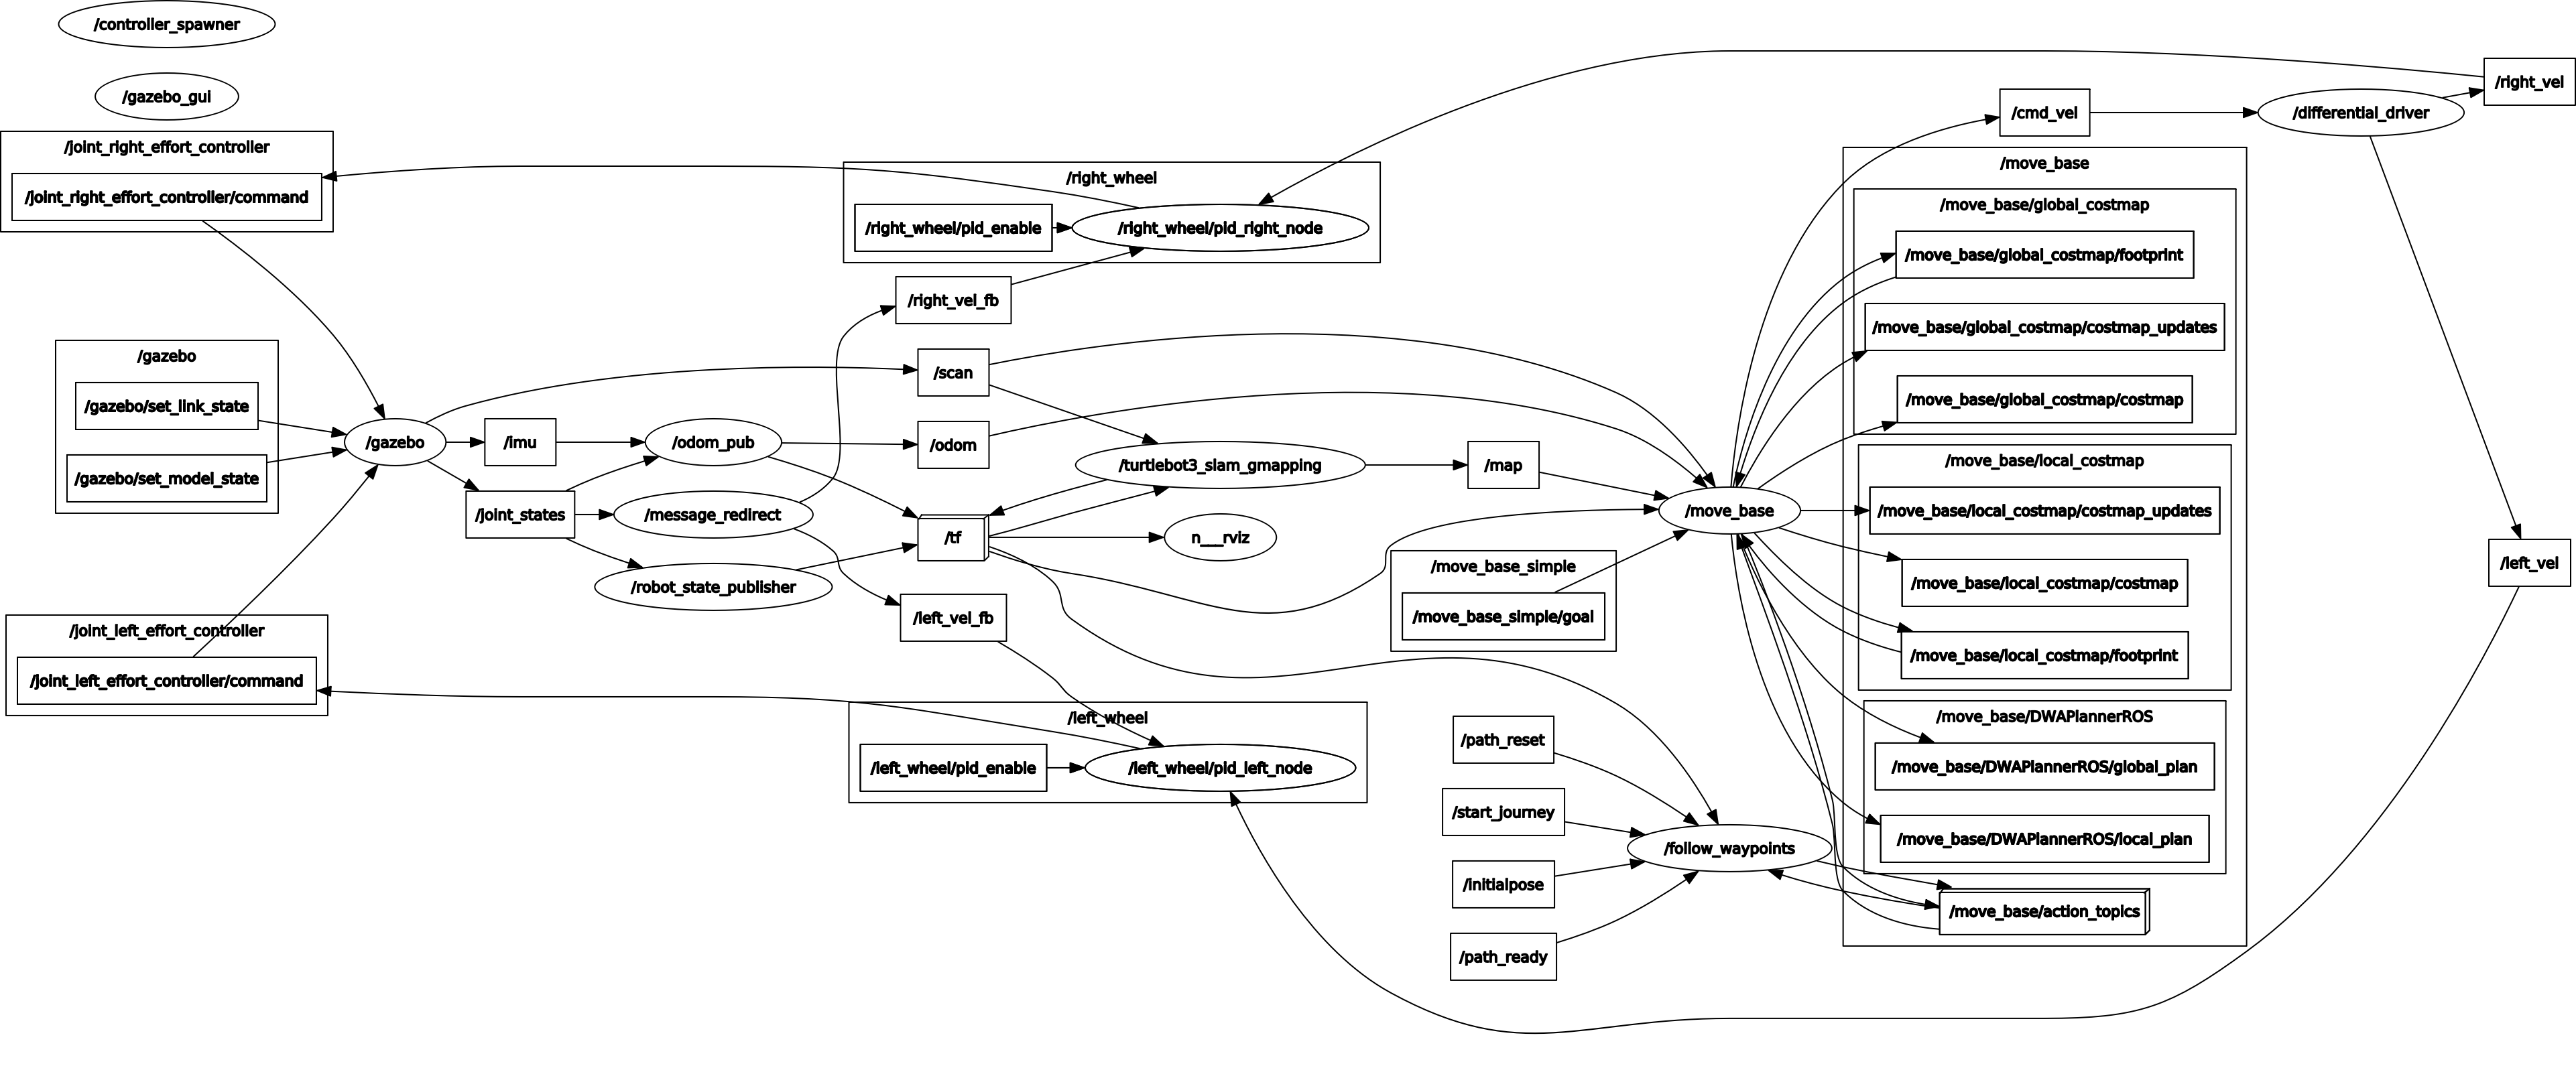
\includegraphics[width=\columnwidth]{images/rosgraph.png}
\end{figure}
\end{landscape}
\begin{landscape}
\newpage
\begin{figure}
    \centering
    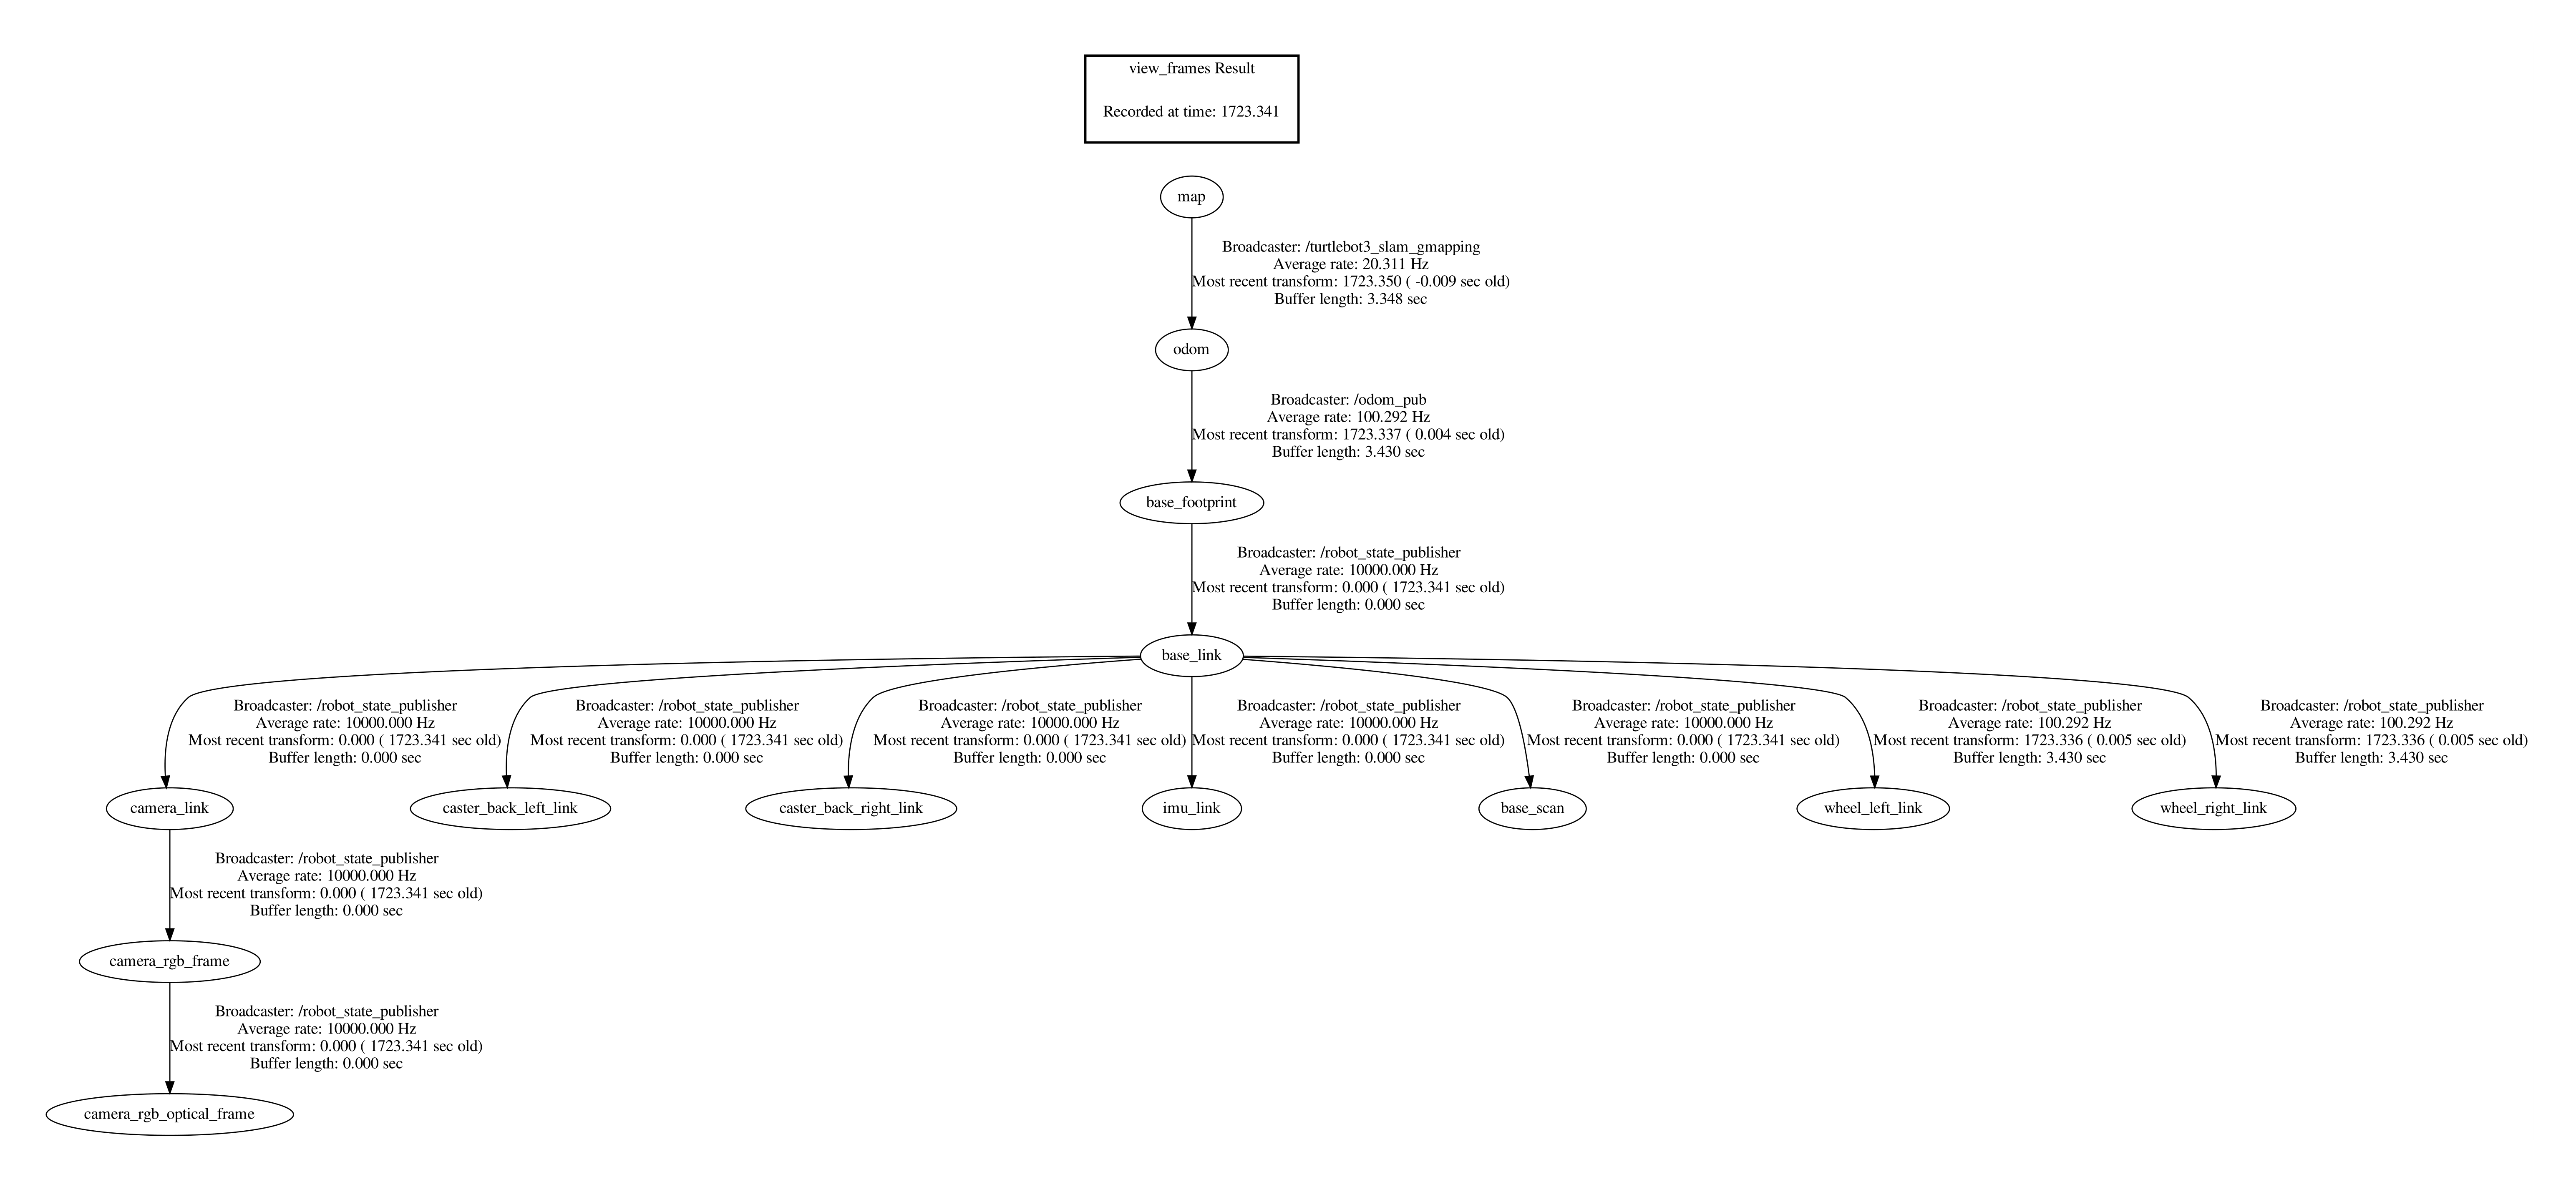
\includegraphics[width=\columnwidth]{images/frames-1.png}
\end{figure}

\end{landscape}
\newpage
\section{Transferring PID Controller to SBC [Experimental Future Work]}
The entire path planning and navigation responsibility is taken care of by the Remote PC in the current configuration of the software. The performance of the software is really good, and no network latency issues were identified. However, it is possible to transfer the control software from the Remote PC to the SBC. \textbf{This implementation has not been tested to work on the TurtleBot3.} Transferring any software from Remote PC to SBC requires three things:
\begin{itemize}
	\item{Compiling custom packages, if any, associated with that software in the same workspace of the stock packages.}	
	\item{Installing required dependencies on the SBC, \ul{if they are available for the linux distro and ROS version running on the TurtleBot SBC.}}
	\item{Changing the \texttt{*.launch} files on the remote PC and SBC}
\end{itemize}
The control on the TurtleBot3 is achieved through the package \texttt{ros\_control}. To run the controller on the SBC, copy the package to the \texttt{catkin\_ws} folder on the SBC. The dependencies required for the package are listed  in the \texttt{CMakeLists.txt} file.
\lstinputlisting[style=XML, firstline=10, lastline=18]{../src/ros_control/CMakeLists.txt}
Finally re-compile the workspace by running \texttt{catkin\_make} in the base directory (by default,\texttt{~/catkin\_ws/}).\\
In addition to the above dependencies, the SBC should have the \texttt{ros-pid} package installed. Run the following command to install it on the SBC.
\begin{lstlisting}[style=bash]
sudo apt-get install ros-kinetic-pid
\end{lstlisting}
This completes step 1 and 2 of the process. Lastly, we need to modify the appropriate \texttt{*.launch} files. Open \texttt{turtlebot3\_robot.launch} file from the \texttt{turtlebot3\_bringup} package using the following command.
\begin{lstlisting}[style=bash]
rosed turtlebot3_bringup turtlebot3_robot.launch
\end{lstlisting}
The file should look something like this.
\lstinputlisting[style=XML, firstline=1, lastline=13]{../src/turtlebot3/turtlebot3_bringup/launch/turtlebot3_robot.launch}
Add the following line to this file before the end tag \texttt{</launch>}.
\begin{lstlisting}[style=XML]
<include file="$(find ros_control)/launch/turtlebot3_control.launch"/>
\end{lstlisting}
Finally, edit the launch file \texttt{turtlebot3\_physical\_nav\_control.launch} located in the \texttt{turtlebot3\_bringup} package in the Remote PC and remove the following line from the file.
\lstinputlisting[style=XML, firstline=4, lastline=4]{../src/turtlebot3/turtlebot3_bringup/launch/turtlebot3_physical_nav_control.launch}
This should enable \texttt{ros-pid} node and associated custom nodes to run on the SBC.

\end{document}

